\documentclass{ctexart}

\usepackage{geometry}                               % 引入定义版面的宏包
\geometry {a4paper, scale = 0.8}                    % A4纸,缩放80%
\usepackage{hyperref}                               % 引入超链接宏包hyperref
\usepackage{amsmath, amssymb, amsthm, mathtools}    % 引入数学环境的相关宏包
\DeclareMathOperator{\cov}{Cov}                     % 定义协方差符号
\numberwithin{equation}{section}                    % 定义公式的三级编号
\usepackage{multicol}                               % 使用分栏排版宏包
\usepackage{comment}                                % 方便后续使用注释语句
\usepackage{tikz}                                   % 绘制矢量图的宏包
\usepackage{xcolor}                                 % 引入定制颜色的xcolor
\definecolor{LightBlue}{RGB}{226, 247, 254}         % 自定义颜色LightBlue
\usepackage{tcolorbox}                              % 引入tcolorbox宏包
\tcbuselibrary{breakable, most, skins, theorems}    % 调用tcolorbox的库
\newtcolorbox{question}[2][breakable] {             % 定义解答和问题的样式
    colback = LightBlue,
    colframe = cyan, 
    fonttitle = \bfseries,  
    title = #2, #1
}
\newenvironment{solution}{\noindent{\textbf{{\color{cyan}解答}}}\quad}
% \excludecomment{solution}                         % 编译指令隐藏所有解答

\begin{document}
\title{《概率论与数理统计》习题}
\author{郑锦阳}
\date{\today}
\maketitle
\tableofcontents
\section{概率论的基本概念}

\begin{question}{题目2}
    设 $A,B,C$ 为三个事件,用 $A,B,C$ 的运算关系表示下列各事件:
    \begin{itemize}
        \item[(1)] $A$ 发生,$B$ 与 $C$ 不发生.
        \item[(2)] $A$ 与 $B$都发生,而 $C$ 不发生.
        \item[(3)] $A,B,C$ 中至少有一个发生.
        \item[(4)] $A,B,C$ 都发生.
        \item[(5)] $A,B,C$ 都不发生.
        \item[(6)] $A,B,C$ 中不多于一个发生.
        \item[(7)] $A,B,C$ 中不多于两个发生.
        \item[(8)] $A,B,C$ 中至少有两个发生.
    \end{itemize}
\end{question}
\begin{solution}
    \begin{multicols}{4}
        \begin{itemize}
            \item[(1)] $A\overline{BC}$
            \item[(2)] $AB\overline{C}$
            \item[(3)] $A \cup B \cup C$
            \item[(4)] $ABC$
            \item[(5)] $\overline{ABC}$
            \item[(6)] $\overline{AB}\cup\overline{AC}\cup\overline{BC}$ %$\overline{ABC} + A\overline{BC} + \overline{A}B\overline{C} + \overline{AB}C$ 或者
            \item[(7)] $\overline{A}\cup\overline{B}\cup\overline{C}$ %$A\cup\overline{A} - A \cap B \cap C$ 或者 
            \item[(8)] $AB \cup AC \cup BC$ %$\overline{A}BC + A\overline{B}C + AB\overline{C} + ABC$ 或者 
        \end{itemize}
    \end{multicols}
\end{solution}


\begin{question}{题目3}
    \begin{itemize}
        \item [(1)] 设 $A,B,C$ 是三个事件,且 $P(A) = P(B) = P(C) = \dfrac{1}{4}$,$P(AB) = P(BC) = 0$,$P(AC) = \dfrac{1}{8}$,求 $A,B,C$ 至少有一个发生的概率.

        \item [(2)] 已知 $P(A) = \dfrac{1}{2}$,$P(B) = \dfrac{1}{3}$,$P(C) = \dfrac{1}{5}$,$P(AB) = \dfrac{1}{10}$,$P(AC) = \dfrac{1}{15}$,$P(BC) = \dfrac{1}{20}$,$P(ABC) = \dfrac{1}{30}$,求 $A \cup B$,$\overline{A}\overline{B}$,$A \cup B \cup C$,$\overline{A}\overline{B}\overline{C}$,$\overline{A}\overline{B}C$,$\overline{A} \overline{B}\cup C$ 的概率.

        \item [(3)] 已知 $P(A) = \dfrac{1}{2}$,(i)若 $A,B$ 互不相容,求$P(A\overline{B})$,(ii)若$P(AB) = \dfrac{1}{8}$,求 $P(A\overline{B})$.
    \end{itemize}
\end{question}
\begin{solution}
    (1) 根据多个事件的加法公式
    $$
        \begin{aligned}
            P(A \cup B \cup C)
             & = P(A) + P(B) + P(C) - P(AB) - P(AC) - P(BC) + P(ABC)              \\
             & = \frac{1}{4} + \frac{1}{4} + \frac{1}{4}- 0 - \frac{1}{8} - 0 + 0 \\
             & = \frac{5}{8}.
        \end{aligned}
    $$
    (2) (i) 根据概率的加法公式
    $$
        \begin{aligned}
            P(A \cup B)
            = P(A) + P(B) - P(AB)
            = \frac{1}{2} + \frac{1}{3} - \frac{1}{10}
            = \frac{11}{15}.
        \end{aligned}
    $$
    (ii) 根据事件运算的德摩根律
    $$
        \begin{aligned}
            P\left(\overline{AB}\right)
            = P\left(\overline{A \cup B}\right) = 1-P(A \cup B)
            = 1-\frac{11}{15} = \frac{4}{15}.
        \end{aligned}
    $$
    (iii) 根据多个事件的加法公式
    $$
        \begin{aligned}
            P(A \cup B \cup C)
             & = P(A) + P(B) + P(C) - P(AB) - P(AC) - P(BC) + P(ABC)                                \\
             & = \frac{1}{2} + \frac{1}{3} + \frac{1}{5} - \frac{1}{10}-\frac{1}{20} + \frac{1}{30} \\
             & = \frac{17}{20}.
        \end{aligned}
    $$
    (iv) 根据事件运算的德摩根律
    $$
        \begin{aligned}
            P\left(\overline{ABC}\right)
            = P\left(\overline{A \cup B \cup C}\right)
            = 1 - P(A \cup B \cup C)
            = 1 - \frac{17}{20}
            = \frac{3}{20}.
        \end{aligned}
    $$
    (v) 设样本空间为 $S$,利用 $\overline{C} = S - C$ 转化
    $$
        \begin{aligned}
            P(\overline{AB}C)
            = P\left(\overline{AB}(S-\overline{C})\right)
            = P\left(\overline{AB}\right) - P\left(\overline{ABC}\right)
            = \frac{4}{15} - \frac{3}{20}
            = \frac{7}{60}.
        \end{aligned}
    $$
    (vi) 将 $\overline{AB}$ 视作一个事件,根据加法公式
    $$
        \begin{aligned}
            P(\overline{AB}\cup C)
            = P(\overline{AB}) + P(C) - P(\overline{AB}C)
            = \frac{4}{15} + \frac{1}{5} - \frac{7}{60}
            = \frac{7}{20}.
        \end{aligned}
    $$
    (3) 设样本空间为 $S$
    $$
        P(A\overline{B}) = P(A(S-B)) = P(A - AB) = P(A) - P(AB).
    $$
    (i) 因为 $A,B$ 互不相容,所以 $P(AB) = 0$
    $$
        P(A\overline{B}) = P(A) - P(AB) = \frac{1}{2} - 0 = \frac{1}{2}.
    $$
    (ii) 若 $P(AB) = \dfrac{1}{8}$
    $$
        P(A\overline{B})
        = P(A)-P(AB)
        = \frac{1}{2}-\frac{1}{8}
        = \frac{3}{8}.
    $$
\end{solution}

\begin{question}{题目4}
    设 $A,B$ 是两个事件.
    \begin{itemize}
        \item[(1)] 已知 $A\overline{B} = \overline{A}B$,验证 $A=B$.
        \item[(2)] 验证事件 $A$ 和事件 $B$ 恰有一个发生的概率为 $P(A) + P(B) - 2P(AB)$.
    \end{itemize}
\end{question}
\begin{solution}
    (1) 设样本空间为 $S$
    $$
        \begin{aligned}
            A\overline{B}     & = \overline{A}B     \\
            A\left(S-B\right) & = \left(S-A\right)B \\
            A - AB            & = B - AB            \\
            A                 & = B.
        \end{aligned}
    $$
    (2) 设样本空间为 $S$
    $$
        \begin{aligned}
            P\left(\overline{A}B + A\overline{B}\right)
             & = P(\overline{A}B) + P(A\overline{B}) \\
             & = P[(S-A)B] + P[A(S-B)]               \\
             & = P(B - AB) + P(A - AB)               \\
             & = P(A) + P(B) - 2P(AB).
        \end{aligned}
    $$
\end{solution}

\begin{question}{题目6} 在房间里有 10 个人,分别佩戴从 1 号到 10 号的纪念章,任选 3 人记录其纪念章的号码.
    \begin{itemize}
        \item[(1)] 求最小号码为 5 的概率.
        \item[(2)] 求最大号码为 5 的概率.
    \end{itemize}
\end{question}
\begin{solution}
    (1) 事件$A_1$包含的基本事件数为$C_5^2$,$S$ 中基本事件的总数为 $C_{10}^3$
    $$
        P(A_1) = \frac{C_5^2}{C_{10}^3} = \frac{1}{12}.
    $$
    (2) 事件$A_2$包含的基本事件数为$C_4^2$,$S$中基本事件的总数为 $C_{10}^3$
    $$
        P(A_2) = \frac{C_4^2}{C_{10}^3} = \frac{1}{20}.
    $$
\end{solution}

\begin{question}{题目7}
    某油漆公司发出 17 桶油漆,其中白漆 10 桶、黑漆 4 桶、红漆 3 桶,在搬运中所有标签脱落,交货人随意将这些油漆发给顾客. 问一个订货为 4 桶白漆、3 桶黑漆和 2 桶红漆的顾客,能按所订颜色如数得到订货的概率是多少?
\end{question}
\begin{solution}
    事件 $A$ 包含的基本事件数为 $C_{10}^4 C_4^3 C_3^2$,$S$ 中基本事件的总数为 $C_{17}^9$.
    $$
        P(A) = \frac{C_{10}^4 C_4^3 C_3^2}{C_{17}^9} = \frac{252}{2431}.
    $$
\end{solution}

\begin{question}{补充习题}
    某厂家称一批数量为 1000 件的产品的次品率为 5\%. 现从该批产品中有放回地抽取了 30 件,经检验发现有次品 5 件,问该厂家是否谎报了次品率?
\end{question}
\begin{solution}
    若次品率为厂家声称的 5\%,那么当有放回地抽检 30 件时,出现次品的数量应为
    $$
        30 \times 5\%  = 1.5.
    $$
    而实际抽检出 5 个次品,这说明厂家谎报了次品率.
    \paragraph{方法二} 假设商家如实地上报次品率,那么有放回地抽取 30 件,出现 5 件次品的概率为
    $$
        P = C_{30}^{5}(5\%)^5(1-5\%)^{25} \approx 0.01235.
    $$
    这是一个很低概率的事件,说明厂家谎报了次品率.
\end{solution}

\begin{question}{题目8}
    在 1500 件产品中有 400 件次品、1100 件正品. 任取 200 件.
    \begin{itemize}
        \item [(1)] 求恰有 90 件次品的概率.
        \item [(2)] 求至少有 2 件次品的概率.
    \end{itemize}
\end{question}
\begin{solution}
    (1) 设事件 $A_1$ 为恰有 90 件次品
    $$
        P(A_1) = \frac{C_{400}^{90}C_{1100}^{110}}{C_{1500}^{200}}.
    $$
    (2) 设事件 $A_2$ 为至少有 2 件次品,考虑其对立事件 $\overline{A_2} = \{ \{\text{没有次品}\}, \{\text{只有1件次品}\} \}$
    $$
        P(A_2) = 1 - P(\overline{A_2})
        = 1 - \frac{C_{400}^{0}C_{1100}^{200}}{C_{1500}^{200}} - \frac{C_{400}^{1}C_{1100}^{199}}{C_{1500}^{200}}.
    $$
\end{solution}

\begin{question}{题目11}
    将 3 只球随机地放入 4 个杯子中去,求杯子中球的最大个数分别为 1,2,3 的概率.
\end{question}
\begin{solution}
    设杯中最多有 $i$ 个球为事件 $A_i$
    $$
        P(A_1) = \frac{C_4^1C_3^1C_2^1}{C_4^1C_4^1C_4^1} = \frac{6}{16}.
    $$
    $$
        P(A_2) = \frac{C_3^2C_4^1C_3^1}{C_4^1C_4^1C_4^1} = \frac{9}{16}.
    $$
    $$
        P(A_3) = \frac{C_4^1}{C_4^1C_4^1C_4^1} = \frac{1}{16}.
    $$
\end{solution}

\begin{question}{题目14}
    \begin{itemize}
        \item [(1)] 已知 $P(\overline{A}) = 0.3$,$P(B) = 0.4$,$P(A\overline{B}) = 0.5$,求条件概率 $P(B|A \cup \overline{B})$.
        \item [(2)] 已知 $P(A) = \dfrac{1}{4}$,$P(B|A) = \dfrac{1}{3}$,$P(A|B) = \dfrac{1}{2}$,求 $P(A \cup B)$.
    \end{itemize}
\end{question}
\begin{solution}
    (1) 根据题设条件,有
    $$
        \begin{cases}
            P(\overline{A}) = 1 - P(A) = 0.3,      \\
            P(B) = 1 - P(\overline{B}) = 0.4,      \\
            P(A\overline{B}) = P(A) - P(AB) = 0.5. \\
        \end{cases}
        \implies
        \begin{cases}
            P(A) = 0.7,            \\
            P(\overline{B}) = 0.6, \\
            P(AB) = 0.2.           \\
        \end{cases}
    $$
    再根据条件概率公式和事件运算的分配律,有
    $$
        P(B|A\cup\overline{B})
        = \frac{P(B(A\cup\overline{B}))}{P(A\cup\overline{B})}
        = \frac{P(BA \cup B\overline{B})}{P(A\cup\overline{B})}
        = \frac{P(AB)}{P(A) + P(\overline{B}) - P(A\overline{B})}
        = \frac{1}{4}.
    $$
    (2) 根据题设条件和乘法定理
    $$
        \begin{cases}
            P(AB) = P(B|A)P(A), \\
            P(AB) = P(A|B)P(B). \\
        \end{cases}
        \implies
        \begin{dcases}
            P(B) = \frac{1}{6},   \\
            P(AB) = \frac{1}{12}. \\
        \end{dcases}
    $$
    进一步有
    $$
        P(A \cup B) = P(A) + P(B) - P(AB) = \frac{1}{3}.
    $$
\end{solution}

\begin{question}{题目16}
    据以往资料表明,某 3 口之家,患某种传染病的概率有以下规律:
    $$
        P\{ \text{孩子得病} \} = 0.6,
    $$
    $$
        P\{ \text{母亲得病}|\text{孩子得病} \} = 0.5,
    $$
    $$
        P\{ \text{父亲得病}|\text{母亲及孩子得病} \} = 0.4,
    $$
    求母亲及孩子得病但父亲未得病的概率.
\end{question}
\begin{solution}
    设样本空间为 $S$,事件 $A$ 为孩子得病,事件 $B$ 为母亲得病,事件 $C$ 为父亲得病
    $$
        \begin{dcases}
            P(A) = 0.6,                           \\
            P(B|A) = \frac{P(AB)}{P(A)} = 0.5,    \\
            P(C|BA) = \frac{P(ABC)}{P(AB)} = 0.4. \\
        \end{dcases}
        \implies
        \begin{cases}
            P(AB) = 0.3,    \\
            P(ABC) =  0.12. \\
        \end{cases}
    $$
    进一步有
    $$
        P(AB\overline{C}) = P(AB(S-C)) = P(AB)-P(ABC) = 0.18.
    $$
\end{solution}

\begin{question}{题目37}
    设第一只盒子中装有 3 只蓝球,2 只绿球,2 只白球;第二只盒子中装有 2 只蓝球,3 只绿球,4只白球. 独立地分别在两只盒子中各取一只球.
    \begin{itemize}
        \item [(1)] 求至少有一只蓝球的概率.
        \item [(2)] 求有一只蓝球、一只白球的概率.
        \item [(3)] 已知至少有一只蓝球,求有一只蓝球一只白球的概率.
    \end{itemize}
\end{question}
\begin{solution}
    (1) 设事件 $A$ 为至少有一只蓝球,考虑其对立事件 $\overline{A}$
    $$
        P(A) = 1-P(\overline{A})
        = 1 - \frac{C_4^1}{C_7^1} \frac{C_7^1}{C_9^1}
        = \frac{5}{9}.
    $$
    (2) 设事件 $B$ 为取出一只蓝球和一只白球
    $$
        P(B) = \frac{C_3^1 C_4^1}{C_7^1C_9^1} + \frac{C_2^1C_2^1}{C_7^1C_9^1}
        = \frac{16}{63}.
    $$
    (3) 根据(1)(2)题的结论和条件概率公式
    $$
        P(B|A) = \frac{P(AB)}{P(A)}
        = \frac{16/63}{5/9}
        = \frac{16}{35}.
    $$
\end{solution}
\section{随机变量及其分布}

\begin{question}{补充习题}
    设某便利店一天中的顾客人数服从参数为 10 的泊松分布,并且这些到店顾客的购物行为彼此独立,其购物概率为 0.6,求每天到便利店且购物的顾客人数的分布.
\end{question}
\begin{solution}
    我们约定用随机变量 $X$ 表示到店的人数,$Y$ 表示到店且购物的人数. 设当天有 $r (r=0, 1, 2, \cdots)$位顾客到店,其中 $k (k \leqslant r)$ 位顾客在到店后选择购物,那么
    $$
        P\{Y=k|X=r\} = C_r^k(0.6)^k(1-0.6)^{r-k}.
    $$
    再根据全概率公式
    $$
        \begin{aligned}
            P\{Y=k\}
             & = \sum_{r=k}^{\infty} P\{Y=k|X=r\} P\{X=r\}                                                 \\
             & = \sum_{r=k}^{\infty} C_r^k(0.6)^k(1-0.6)^{r-k} \frac{10^r\mathrm{e}^{-10}}{r!}             \\
             & = \sum_{r=k}^{\infty} \frac{r!}{k!(r-k)!}(0.6)^k(0.4)^{r-k}\frac{10^r\mathrm{e}^{-10}}{r!}. \\
        \end{aligned}
    $$
    约去 $r!$ 后,进一步令 $r-k=i$
    $$
        \begin{aligned}
            P\{Y=k\}
             & = \sum_{i=0}^{\infty} \frac{1}{k!i!}(0.6)^k(0.4)^{i}10^{i+k}\mathrm{e}^{-10}  \\
             & = \frac{0.6^k10^k\mathrm{e}^{-10}}{k!}\sum_{i=0}^{\infty}\frac{0.4^i10^i}{i!} \\
             & = \frac{6^k\mathrm{e}^{-10}}{k!} \sum_{i=0}^{\infty}\frac{4^i}{i!}            \\
             & = \frac{6^k\mathrm{e}^{-6}}{k!}.
        \end{aligned}
    $$
\end{solution}

\begin{question}{题目2}
    \begin{itemize}
        \item [(1)] 一袋中装有 5 只球,编号为 1,2,3,4,5. 在袋中同时取 3 只,以 $X$ 表示取出的 3 只球中的最大号码,写出随机变量 $X$ 的分布律.
        \item [(2)] 将一颗骰子抛掷两次,以 $X$ 表示两次中得到的小的点数,试求 $X$ 的分布律.
    \end{itemize}
\end{question}
\begin{solution}
    (1) 随机变量 $X$ 的取值范围为 $3, 4, 5$
    $$
        \begin{aligned}
            P\{X = 3\} = \frac{C_2^2}{C_5^3} = \frac{1}{10}, \\
            P\{X = 4\} = \frac{C_3^2}{C_5^3} = \frac{3}{10}, \\
            P\{X = 5\} = \frac{C_4^2}{C_5^3} = \frac{6}{10}.
        \end{aligned}
    $$
    其分布律为
    $$
        \renewcommand\arraystretch{2}
        \setlength{\arraycolsep}{6mm}
        \begin{array}{c|ccc}
            X   & 3             & 4             & 5             \\
            \hline
            p_k & \dfrac{1}{10} & \dfrac{3}{10} & \dfrac{6}{10}
        \end{array}
    $$
    (2) 随机变量 $X$ 的取值范围为 $1, 2, 3, 4, 5, 6$
    $$
        P\{X=1\} = A_2^2\frac{C_5^1}{C_6^1C_6^1} + \frac{1}{C_6^1C_6^1} = \frac{11}{36},
    $$
    $$
        P\{X=2\} = A_2^2\frac{C_4^1}{C_6^1C_6^1} + \frac{1}{C_6^1C_6^1} = \frac{9}{36},
    $$
    $$
        P\{X=3\} = A_2^2\frac{C_3^1}{C_6^1C_6^1} + \frac{1}{C_6^1C_6^1} = \frac{7}{36},
    $$
    $$
        P\{X=4\} = A_2^2\frac{C_2^1}{C_6^1C_6^1} + \frac{1}{C_6^1C_6^1} = \frac{5}{36},
    $$
    $$
        P\{X=5\} = A_2^2\frac{C_1^1}{C_6^1C_6^1} + \frac{1}{C_6^1C_6^1} = \frac{3}{36},
    $$
    $$
        P\{X=6\} = \frac{1}{C_6^1C_6^1} = \frac{1}{36}.
    $$
    其分布律为
    $$
        \renewcommand\arraystretch{2}
        %\setlength{\arraycolsep}{6mm}
        \begin{array}{c|cccccc}
            X   & 1              & 2             & 3             & 4             & 5             & 6             \\
            \hline
            p_k & \dfrac{11}{36} & \dfrac{9}{36} & \dfrac{7}{36} & \dfrac{5}{36} & \dfrac{3}{36} & \dfrac{1}{36} \\
        \end{array}
    $$
\end{solution}

\begin{question}{题目6}
    大楼装有 5 台同类型的供水设备. 设各台设备是否被使用相互独立. 调查表明在任一时刻 $t$ 每台设备被使用的概率为0.1,问在同一时刻,
    \begin{itemize}
        \item [(1)] 恰有 $2$ 台设备被使用的概率是多少?
        \item [(2)] 至少有 $3$ 台设备被使用的概率是多少?
        \item [(3)] 至多有 $3$ 台设备被使用的概率是多少?
        \item [(4)] 至少有 $1$ 台设备被使用的概率是多少?
    \end{itemize}
\end{question}
\begin{solution}
    我们约定随机变量 $X$ 为正在被使用的设备数量,其分布列为
    $$
        P\{X = k\} = C_5^k(0.1)^k(1-0.1)^{5-k},(k = 0, 1, 2, 3, 4, 5)
    $$
    $$
        \begin{array}{c|ccccccc}
            X   & 0       & 1       & 2      & 3      & 4       & 5       \\
            \hline
            p_k & 0.59049 & 0.32805 & 0.0729 & 0.0081 & 0.00045 & 0.00001
        \end{array}
    $$
    (1) 恰有 2 台设备被使用的概率
    $$
        P\{X=2\} = C_5^2(0.1)^2(0.9)^3 = 0.0729.
    $$
    (2)至少有 3 台设备被使用的概率
    $$
        P\{X \geqslant 3\} = \sum_{k=3}^5 p_k = 0.00856.
    $$
    (3) 至多有 3 台设备被使用的概率
    $$
        P\{X \leqslant 3\} = \sum_{k=0}^3 p_k = 0.99954.
    $$
    (4) 至少有 1 台设备被使用的概率
    $$
        P\{X \geqslant 1\} = \sum_{k=1}^5 p_k = 0.40951.
    $$
\end{solution}

\begin{question}{题目14}
    某人家中在时间间隔 $t$ (以h计)内接到电话的次数 $X$ 服从参数为 $2t$ 的泊松分布.
    \begin{itemize}
        \item [(1)] 若他外出计划用时 10min ,问其间有电话铃响一次的概率是多少?
        \item [(2)] 若他希望外出时没有电话的概率至少为 0.5,问他外出应控制最长时间是多少?
    \end{itemize}
\end{question}
\begin{solution}
    (1) 当他外出 $t = \dfrac{1}{6}$ h时,其间电话铃响 $k=1$ 次的概率
    $$
        P\{X=1\} = \frac{(2t)^1\mathrm{e}^{-2t}}{1!}
        = \frac{1}{3}\mathrm{e}^{-\frac{1}{3}}.
    $$
    (2) 他外出时没有电话的概率至少为 0.5
    $$
        P\{X=0\} = \frac{(2t)^0\mathrm{e}^{-2t}}{0!} \geqslant 0.5.
    $$
    解得最长的外出时间为 $t \leqslant \dfrac{\ln2}{2} \,\mathrm{h}$.
\end{solution}


\begin{question}{题目16}
    有一繁忙的汽车站,每天有大量汽车通过,设一辆汽车在一天的某段时间内出事故的概率为 0.0001. 在某天的该时间段内有 1000 辆汽车通过. 问出事故的车辆数不小于 2 的概率是多少?(利用泊松定理计算)
\end{question}
\begin{solution}
    用随机变量 $X$ 表示出事故的车辆数,且 $X \sim \pi(\lambda)$,其中$\lambda = np = 0.1$
    $$
        \begin{aligned}
            P\{ X \geqslant 2\}
             & = 1 - P\{X=0\} - P\{X=1\}                                                   \\
             & = 1 - \frac{0.1^0\mathrm{e}^{-0.1}}{0!} - \frac{0.1^1\mathrm{e}^{-0.1}}{1!} \\
             & \approx 0.00468.
        \end{aligned}
    $$
\end{solution}


\begin{question}{题目17}
    \begin{itemize}
        \item [(1)] 设 $X$ 服从 $(0-1)$ 分布,其分布律为 $P\{X=k\} = p^k(1-p)^{1-k},(k=0,1)$. 求 $X$ 的分布函数,并作出其图形.
        \item [(2)] 求第2题(1)中的随机变量的分布函数.
    \end{itemize}
\end{question}
\begin{solution}
    (1) 根据 $P\{X=0\} = 1-p$,$P\{X=1\} = p$ ,得到分布函数 $F(x)$
    $$
        F(x) = \begin{cases}
            0,   & x <0,              \\
            1-p, & 0 \leqslant x < 1, \\
            1,   & x \geqslant 1.
        \end{cases}
    $$
    作出分布函数图形
    \begin{center}
        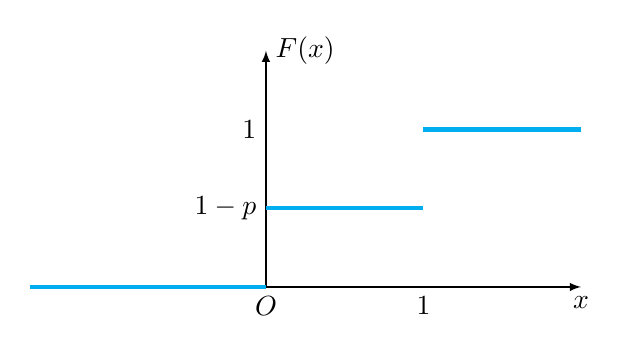
\begin{tikzpicture}[scale = 2]
            %画出x轴,并标注(1,0)
            \draw[-latex] (-1.5,0) -- (2,0) node[below]{$x$};
            \node[left] at (0,1) {$1$} ;
            %画出F(x)轴,并标注(0,0) (0,1) (0,1-p)
            \draw[-latex] (0, 0) -- (0, 1.5) node[right]{$F(x)$};
            \node[below] at (1,0) {$1$};
            \node[left] at (0,0.5) {$1-p$};
            \node[below] at (0,0) {$O$};

            %画出分段的分布函数F(x)
            \draw[cyan, line width = 1.5pt] (-1.5, 0) -- (0, 0);
            \draw[cyan, line width = 1.5pt] (0, 0.5) -- (1, 0.5);
            \draw[cyan, line width = 1.5pt] (1, 1) -- (2, 1);
            %标注虚线连续
            %\draw[dashed, cyan] (0,0) -- (0,0.5);
            %\draw[dashed, cyan] (1,0.5) -- (1,1);
            %标注两个实心连续点
            %\fill[cyan ] (0, 0.5) circle (0.5pt);
            %\fill[cyan ] (1,   1) circle (0.5pt);
            %标注两个空心间断点
            %\draw[cyan ] (0,   0) circle (0.5pt);
            %\fill[white] (0,   0) circle (0.5pt);
            %\draw[cyan ] (1, 0.5) circle (0.5pt);
            %\fill[white] (1, 0.5) circle (0.5pt);
        \end{tikzpicture}
    \end{center}
    (2) 分布函数为
    $$
        F(x) = \begin{dcases}
            0,            & x < 3,             \\
            \frac{1}{10}, & 3 \leqslant x < 4, \\
            \frac{4}{10}, & 4 \leqslant x < 5, \\
            1,            & x \geqslant 5 .
        \end{dcases}
    $$
\end{solution}

\begin{question}{题目20}
    设随机变量 $X$ 的分布函数为
    $$
        F_X(x) = \begin{cases}
            0,      & x<1,                        \\
            \ln{x}, & 1 \leqslant x < \mathrm{e}, \\
            1,      & x \geqslant \mathrm{e}.
        \end{cases}
    $$
    \begin{itemize}
        \item[(1)] 求 $P\{X<2\}$ , $P\{0 < X \leqslant 3\}$ , $P\left\{2 < X < \dfrac{5}{2}\right\}$.
        \item[(2)] 求概率密度 $f_X(x)$.
    \end{itemize}
\end{question}
\begin{solution}
    (1) 根据分布函数的定义
    $$
        P\{X<2\} = F(2) = \ln2.
    $$
    $$
        P\{0 < X \leqslant 3\}
        = P\{X \leqslant 3\} - P\{X \leqslant 0\}
        = F(3) - F(0)
        = 1.
    $$
    $$
        P\left\{2 < X < \frac{5}{2}\right\}
        = P\left\{X<\frac{5}{2}\right\} - P\{X<2\}
        = F\left(\frac{5}{2}\right) - F(2)
        = \ln\frac{5}{4}.
    $$
    (2) 概率密度为
    $$
        f_X(x) = F'_X(x) = \begin{dcases}
            \frac{1}{x}, & 1 \leqslant x < \mathrm{e}, \\
            0,           & \text{其他}.
        \end{dcases}
    $$
\end{solution}


\begin{question}{题目24}
    设顾客在某银行的窗口的等待服务的时间 $X$(min) 服从指数分布,其概率密度为
    $$
        f_X(x) = \begin{dcases}
            \frac{1}{5}\mathrm{e}^{-\frac{x}{5}}, & x>0,         \\
            0,                                    & \text{其他}.
        \end{dcases}
    $$
    某顾客在窗口等待服务,若超过10min他就离开. 他一个月要到银行 $5$ 次. 以 $Y$ 表示一个月内他未等到服务而离开窗口的次数. 写出 $Y$ 的分布律,并求$P\{Y \geqslant 1\}$.
\end{question}
\begin{solution}
    随机变量 $X$ 的分布函数为
    $$
        F_X(x)
        = \int_{-\infty}^{x} f(x) \,\mathrm{d}x
        = \int_{0}^{x} \frac{1}{5}\mathrm{e}^{-\frac{x}{5}} \mathrm{d}x
        = \begin{cases}
            1-\mathrm{e}^{-\frac{x}{5}}, & x>0,         \\
            0,                           & \text{其他}.
        \end{cases}
    $$
    顾客在银行等待时间大于 $10$min 的概率为
    $$
        P\{X>10\} = 1 - P\{X \leqslant 10\}
        = 1 - \left(1-\mathrm{e}^{-2}\right)
        = \mathrm{e}^{-2}.
    $$
    设一个月内顾客有 $k$次因为等待超时而离开窗口,那么 $Y$ 的分布律为
    $$
        P\{Y=k\} = C_5^k\left(\mathrm{e}^{-2}\right)^{k}\left(1-\mathrm{e}^{-2}\right)^{5-k} (k=0,1,2,3,4,5).
    $$
    进一步得到
    $$
        P\{Y \geqslant 1\}
        = 1 - P\{Y=0\}
        = 1 - \left(1-\mathrm{e}^{-2}\right)^5
        \approx 0.5167.
    $$
\end{solution}


\begin{question}{题目27}
    某地区 18 岁的女青年的血压(收缩压以mmHg计)服从 $N(110,12^2)$分布. 在该地区任选一 18 岁的女青年,测量她的血压 $X$. 求
    \begin{itemize}
        \item[(1)] $P\{X \leqslant 105\}$,$P\{100 < X \leqslant 120\}$.
        \item[(2)] 确定最小的 $x$,使 $P\{X>x\} \leqslant 0.05$.
    \end{itemize}
\end{question}
\begin{solution}
    (1) 把正态分布线性变换成标准正态分布,得到
    $$
        \begin{aligned}
            P\{X \leqslant 105\}
             & = P\left\{\frac{X-110}{12} \leqslant \frac{105-110}{12}\right\} \\
             & = \Phi\left(-\frac{5}{12}\right)                                \\
             & = 1 - \Phi\left(\frac{5}{12}\right)                             \\
             & \approx 0.3385.
        \end{aligned}
    $$
    $$
        \begin{aligned}
            P\left\{100 < X \leqslant 120\right\}
             & = P\left\{\frac{100-110}{12} < \frac{X-110}{12} \leqslant \frac{120-110}{12}\right\} \\
             & = \Phi\left(\frac{5}{6}\right) - \Phi\left(-\frac{5}{6}\right)                       \\
             & = 2\Phi\left(\frac{5}{6}\right) - 1                                                  \\
             & \approx 0.5953.
        \end{aligned}
    $$
    (2) 题意等价为 $1 - P\{X \leqslant x\} \leqslant 0.05$ ,再把正态分布线性变换成标准正态分布,得到
    $$
        \begin{aligned}
            P\{X \leqslant x\}                                          & \geqslant 0.95 \\
            P\left\{\frac{X-110}{12} \leqslant \frac{x-110}{12}\right\} & \geqslant 0.95 \\
            \Phi\left(\frac{x-110}{12}\right)                           & \geqslant 0.95 \\
        \end{aligned}
    $$
    查表得到 $\left(\dfrac{x-110}{12}\right)_{\min} = 1.65$,也即 $x_{\min} = 129.8$.
\end{solution}

\begin{question}{题目33}
    设随机变量 $X$ 的分布律为
    $$
        \renewcommand\arraystretch{2}
        \setlength{\arraycolsep}{6mm}
        \begin{array}{c|ccccc}
            X   & -2           & -1           & 0            & 1             & 3              \\
            \hline
            p_k & \dfrac{1}{5} & \dfrac{1}{6} & \dfrac{1}{5} & \dfrac{1}{15} & \dfrac{11}{30} \\
        \end{array}
    $$
    求 $Y=X^2$ 的分布律.
\end{question}
\begin{solution}
    根据
    $$
        P\{Y=0\} = P\{X=0\} = \frac{6}{30}.
    $$
    $$
        P\{Y=1\} = P\{X=-1\} + P\{X=1\} = \frac{7}{30}.
    $$
    $$
        P\{Y=4\} = P\{X=-2\} = \frac{6}{30}.
    $$
    $$
        P\{Y=9\} = P\{X=3\} = \frac{11}{30}.
    $$
    得到 $Y$ 的分布律
    $$
        \renewcommand\arraystretch{2}
        \setlength{\arraycolsep}{6mm}
        \begin{array}{c|cccc}
            X   & 0             & 1             & 4             & 9              \\
            \hline
            p_k & \dfrac{6}{30} & \dfrac{7}{30} & \dfrac{6}{30} & \dfrac{11}{30}
        \end{array}
    $$
\end{solution}


\begin{question}{题目34}
    设随机变量 $X$ 在区间 $(0,1)$ 服从均匀分布.
    \begin{itemize}
        \item [(1)] 求 $Y = \mathrm{e}^X$ 的概率密度.
        \item [(2)] 求 $Y = -2\ln{X}$ 的概率密度.
    \end{itemize}
\end{question}
\begin{solution}
    随机变量 $X$ 在区间 $(0,1)$ 服从均匀分布,概率密度为
    $$
        f(x) = \begin{cases}
            1, & 0<x<1,       \\
            0, & \text{其他}.
        \end{cases}
    $$
    (1) 根据 $Y = \mathrm{e}^X$,得到 $Y$ 的分布函数
    $$
        F_Y(y)
        = P\{Y \leqslant y\}
        = P\left\{\mathrm{e}^X \leqslant y\right\}
        = P\left\{X \leqslant \ln{y}\right\}
        = F_X(\ln{y}).
    $$
    将 $F_Y(y)$ 对 $y$ 求导,得到 $Y = \mathrm{e}^X$ 的概率密度
    $$
        f_Y(y) = F_X'(\ln{y}) = f_X(\ln{y}) \cdot \ln'{y}
        = \begin{dcases}
            \frac{1}{y}, & 0 < \ln{y} < 1, \\
            0,           & \text{其他}.
        \end{dcases}
        = \begin{dcases}
            \frac{1}{y}, & 1 < y < \mathrm{e}, \\
            0,           & \text{其他}.
        \end{dcases}
    $$
    (2) 根据 $Y = -2\ln{X}$,得到 $Y$ 的分布函数
    $$
        F_Y(y)
        = P\{Y \leqslant y\}
        = P\left\{X \geqslant \mathrm{e}^{-\frac{y}{2}}\right\}
        = 1 - P\left\{X < \mathrm{e}^{-\frac{y}{2}}\right\}
        = 1 - F_X\left(\mathrm{e}^{-\frac{y}{2}}\right).
    $$
    将 $F_Y(y)$ 对 $y$ 求导,得到 $Y = -2\ln{X}$ 的概率密度
    $$
        f_Y(y)
        = \left[1 - F_X\left(\mathrm{e}^{-\frac{y}{2}}\right)\right]'
        = -f_X\left(\mathrm{e}^{-\frac{y}{2}}\right) \left(\mathrm{e}^{-\frac{y}{2}}\right)'
        = \begin{dcases}
            \frac{1}{2}\mathrm{e}^{-\frac{y}{2}}, & 0<\mathrm{e}^{-\frac{y}{2}}<1, \\
            0,                                    & \text{其他}.
        \end{dcases}
        = \begin{dcases}
            \frac{1}{2}\mathrm{e}^{-\frac{y}{2}}, & y>0,         \\
            0,                                    & \text{其他}.
        \end{dcases}
    $$
\end{solution}


\begin{question}{题目35}
    设 $X \sim N(0,1)$.
    \begin{itemize}
        \item [(1)] 求 $Y=\mathrm{e}^X$ 的概率密度.
        \item [(2)] 求 $Y=2X^2 + 1$ 的概率密度.
        \item [(3)] 求 $Y=|X|$ 的概率密度.
    \end{itemize}
\end{question}
\begin{solution}
    随机变量 $X \sim N(0,1)$ ,其概率密度为
    $$
        f(x) = \frac{1}{\sqrt{2\pi}}\mathrm{e}^{-\frac{x^2}{2}}.
    $$
    (1) 根据 $Y = \mathrm{e}^X$ 得到 $Y$ 的分布函数
    $$
        F_Y(y)
        = P\{Y \leqslant y\}
        = P\{\mathrm{e}^X \leqslant y\}
        = P\{X \leqslant \ln y\}
        = F_X(\ln{y}).
    $$
    将 $F_Y(y)$ 对 $y$ 求导,得到 $Y=\mathrm{e}^X$ 的概率密度
    $$
        \begin{aligned}
            f_Y(y)
            = F_X'(\ln{y}) = f_X(\ln{y})\cdot\frac{1}{y}
            = \begin{dcases}
                  \frac{1}{\sqrt{2\pi}y}\mathrm{e}^{-\frac{\ln^2y}{2}}, & y > 0,         \\
                  0 ,                                                   & y \leqslant 0.
              \end{dcases}
        \end{aligned}
    $$
    (2) 根据 $Y=2X^2+1$ 得到 $Y$ 的分布函数
    $$
        \begin{aligned}
            F_Y(y)
             & = P\{Y \leqslant y\} = P\{2X^2+1 \leqslant y\}                                     \\
             & = P\left\{-\sqrt{\frac{y-1}{2}} \leqslant X \leqslant \sqrt{\frac{y-1}{2}}\right\} \\
             & = F_X\left(\sqrt{\frac{y-1}{2}}\right) - F_X\left(-\sqrt{\frac{y-1}{2}}\right).    \\
        \end{aligned}
    $$
    将 $F_Y(y)$ 对 $y$ 求导,得到 $Y = 2X^2+1$ 的概率密度
    $$
        \begin{aligned}
            f_Y(y)
             & = F_X'\left(\sqrt{\frac{y-1}{2}}\right)
            - F_X'\left(\sqrt{\frac{y-1}{2}}\right)                                              \\
             & = f_X\left(\sqrt{\frac{y-1}{2}}\right)\left(\sqrt{\frac{y-1}{2}}\right)'
            - f_X\left(-\sqrt{\frac{y-1}{2}}\right)\left(-\sqrt{\frac{y-1}{2}}\right)'           \\
             & = \begin{dcases}
                     \frac{1}{2\sqrt{\pi(y-1)}}\mathrm{e}^{-\frac{y-1}{4}}, & y \geqslant 1, \\
                     0,                                                     & \text{其他}.
                 \end{dcases}
        \end{aligned}
    $$
    (3) 根据 $Y=|X|$ 得到 $Y$ 的分布函数
    $$
        F_Y(y) = P\{Y \leqslant y\}
        = P\{|X| \leqslant y\}
        = P\{-y \leqslant X \leqslant y\}
        = F_X(y) - F_X(-y).
    $$
    将 $F_Y(y)$ 对 $y$ 求导,得到 $Y = |X|$ 的概率密度
    $$
        f_Y(y) = F_X'(y) - F_X'(-y)
        = f_X(y) - [-f_X(-y)]
        = \begin{dcases}
            \sqrt{\frac{2}{\pi}}\mathrm{e}^{-\frac{y^2}{2}}, & y \geqslant 0, \\
            0,                                               & \text{其他}.
        \end{dcases}
    $$
\end{solution}
\section{多维随机变量及其分布}

\begin{question}{题目1}
    在一箱子中装有 12 只开关,其中 2 只是次品,在其中取两次,每次任取一只,考虑两种试验:(1)放回抽样,(2)不放回抽样. 我们定义随机变量 $X,Y$ 如下:
    $$
        X = \begin{cases}
            0, & \text{若第一次取出的是正品}, \\
            1, & \text{若第一次取出的是次品},
        \end{cases}
        \quad
        Y = \begin{cases}
            0, & \text{若第二次取出的是正品}, \\
            1, & \text{若第二次取出的是次品}.
        \end{cases}
    $$
    试分别就 (1)(2) 两种情况,写出 $X$ 和 $Y$ 的联合分布律.
\end{question}
\begin{solution}
    (1) 进行放回抽样时
    $$
        P\{X=0,Y=0\}
        = \frac{C_{10}^1C_{10}^1}{C_{12}^1C_{12}^1}
        = \frac{25}{36}.
    $$
    $$
        P\{X=0,Y=1\}
        = \frac{C_{10}^1C_{2}^1}{C_{12}^1C_{12}^1}
        = \frac{5}{36}.
    $$
    $$
        P\{X=1,Y=0\}
        = \frac{C_2^1C_{10}^1}{C_{12}^1C_{12}^1}
        = \frac{5}{36}.
    $$
    $$
        P\{X=1,Y=1\}
        = \frac{C_2^1C_2^1}{C_{12}^1C_{12}^1}
        = \frac{1}{36}.
    $$
    进一步,得到 $X$ 和 $Y$ 的联合分布律:
    $$
        %\renewcommand\arraystretch{2}
        %\setlength{\arraycolsep}{12mm}
        \begin{array}{c|cc|c}
            Y \setminus X & 0     & 1    & P\{Y=j\} \\
            \hline
            0             & 25/36 & 5/36 & 30/36    \\
            1             & 5/36  & 1/36 & 6/36     \\
            \hline
            P\{X=i\}      & 30/36 & 6/36 & 1        \\
        \end{array}
    $$
    (2) 进行不放回抽样时
    $$
        P\{X=0,Y=0\}
        = \frac{C_{10}^1C_9^1}{C_{12}^1C_{11}^1}
        = \frac{45}{66},
    $$
    $$
        P\{X=0,Y=1\}
        = \frac{C_{10}^1C_2^1}{C_{12}^1C_{11}^1}
        = \frac{10}{66},
    $$
    $$
        P\{X=1,Y=0\}
        = \frac{C_2^1C_{10}^1}{C_{12}^1C_{11}^1}
        = \frac{10}{66},
    $$
    $$
        P\{X=1,Y=1\}
        = \frac{C_2^1C_1^1}{C_{12}^1C_{11}^1}
        = \frac{1}{66}.
    $$
    进一步,得到 $X$ 和 $Y$ 的联合分布律:
    $$
        %\renewcommand\arraystretch{1.8}
        %\setlength{\arraycolsep}{9mm}
        \begin{array}{c|cc|c}
            Y \setminus X & 0     & 1     & P\{Y=j\} \\
            \hline
            0             & 45/66 & 10/66 & 55/66    \\
            1             & 10/66 & 1/66  & 11/66    \\
            \hline
            P\{X=i\}      & 55/66 & 11/66 & 1        \\
        \end{array}
    $$
\end{solution}


\begin{question}{题目2}
    \begin{itemize}
        \item [(1)] 盒子里装有 3 只黑球、2只红球、2只白球,在其中任取4只球. 以 $X$ 表示取到黑球的只数,以 $Y$ 表示取到红球的只数. 求$X$ 和 $Y$ 的联合分布律.
        \item [(2)] 在 (1) 中求 $P\{X>Y\}$,$P\{Y=2X\}$,$P\{X+Y=3\}$,$P\{X<3-Y\}$.
    \end{itemize}
\end{question}
\begin{solution}
    (1)设取出黑球 $k$ ($k=0,1,2,3$) 个,取出红球 $r$($r=0,1,2$) 个,取出白球 $4-k-r$ 个.
    $$
        P\{X=k, Y=r\} = \frac{C_4^kC_2^rC_2^{4-k-r}}{C_7^4}
        (k + r \leqslant 4),
    $$
    进一步,得到 $X$ 和 $Y$ 的联合分布律:
    $$
        %\renewcommand\arraystretch{2}
        %\setlength{\arraycolsep}{6mm}
        \begin{array}{c|cccc|c}
            Y \setminus X & 0    & 1     & 2     & 3    & P\{Y=j\} \\
            \hline
            0             & 0    & 0     & 3/35  & 2/35 & 5/35     \\
            1             & 0    & 6/35  & 12/35 & 2/35 & 20/35    \\
            2             & 1/35 & 6/35  & 3/35  & 0    & 10/35    \\
            \hline
            P\{X=i\}      & 1/35 & 12/35 & 18/35 & 4/35 & 1        \\
        \end{array}
    $$
    (2) 根据(1)题的结论
    $$
        P\{X>Y\} = \frac{19}{35},
    $$
    $$
        P\{Y=2X\} = \frac{6}{35},
    $$
    $$
        P\{X+Y=3\} = \frac{20}{35},
    $$
    $$
        P\{X<3-Y\} = \frac{10}{35}.
    $$
\end{solution}

\begin{question}{题目5}
    设随机变量 $(X,Y)$ 的概率密度为
    $$
        F(x,y) = \begin{cases}
            1-\mathrm{e}^{-x}-\mathrm{e}^{-y}+\mathrm{e}^{-x-y}, & x>0,y>0,     \\
            0,                                                   & \text{其他}.
        \end{cases}
    $$
    求边缘分布函数.
\end{question}
\begin{solution}
    根据边缘分布函数的定义,$X$ 的边缘分布函数为
    $$
        F_X(x) = F(x, +\infty) =
        \begin{cases}
            1 - \mathrm{e}^{-x}, & x>0,         \\
            0,                   & \text{其他}.
        \end{cases}
    $$
    同理,$Y$ 的边缘分布函数为
    $$
        F_Y(y) = F(+\infty, y) =
        \begin{cases}
            1 - \mathrm{e}^{-y}, & y>0,         \\
            0,                   & \text{其他}.
        \end{cases}
    $$
\end{solution}


\begin{question}{题目9}
    设二维随机变量 $(X,Y)$ 的概率密度为
    $$
        f(x,y) = \begin{cases}
            cx^2y, & x^2 \leqslant y \leqslant 1, \\
            0,     & \text{其他}.
        \end{cases}
    $$
    \begin{itemize}
        \item[(1)] 确定常数 $c$.
        \item[(2)] 求边缘概率密度.
    \end{itemize}
\end{question}
\begin{solution}
    (1) 概率密度不为零的区域如图所示
    \begin{center}
        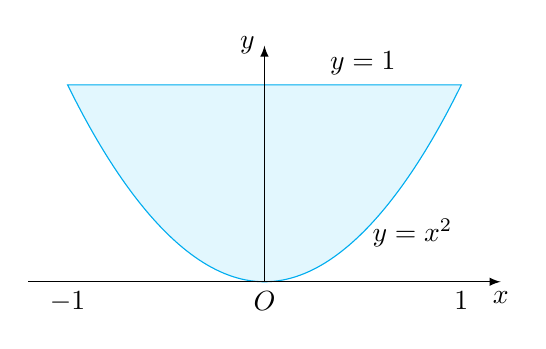
\begin{tikzpicture}[scale = 2.5]
            %画填充色块和边界线
            \filldraw[LightBlue] (-1,1) parabola bend (0,0) (1,1) -- (-1,1) -- cycle;
            \draw[cyan] (-1,1) parabola bend (0,0) (1,1) -- (-1,1) -- cycle;
            %标注边界线的表达式
            \node[right] at (0.5, 0.25) {$y=x^2$};
            \node[above] at (0.5, 1) {$y=1$};
            \node[below] at (1,0) {$1$};
            \node[below] at (-1,0) {$-1$};
            %标注坐标轴
            \draw[-latex] (0, 0) -- (0, 1.2) node[left] {$y$};
            \draw[-latex] (-1.2, 0) -- (1.2, 0) node[below] {$x$};
            \node[below] at (0,0) {$O$};
        \end{tikzpicture}
    \end{center}
    根据概率密度 $f(x,y)$ 的性质
    $$
        \int_{-\infty}^{+\infty}\int_{-\infty}^{+\infty} f(x,y) \,\mathrm{d}x\mathrm{d}y
        = \int_{-1}^1\int_{x^2}^1 cx^2y \,\mathrm{d}x\mathrm{d}y
        = c\int_{-1}^1 x^2\left(\frac{1}{2} - \frac{1}{2}x^4\right)\mathrm{d}x
        = \frac{4}{21}c
        = 1.
    $$
    解得
    $$
        c = \frac{21}{4}.
    $$
    (2) 根据边缘概率密度的定义,$X$的边缘概率密度为
    $$
        f_X(x)
        = \int_{-\infty}^{+\infty} f(x,y) \,\mathrm{d}y
        = \int_{x^2}^{1} \frac{21}{4}x^2y \,\mathrm{d}y
        = \begin{dcases}
            \frac{21}{8}x^2(1-x^4), & -1 \leqslant x \leqslant 1, \\
            0,                      & \text{其他}.
        \end{dcases}
    $$
    同理, $Y$ 的边缘概率密度为
    $$
        f_Y(y) = \int_{-\infty}^{+\infty} f(x,y) \,\mathrm{d}x
        = \int_{-\sqrt{y}}^{\sqrt{y}} \frac{21}{4}x^2y \,\mathrm{d}x
        = \begin{dcases}
            \frac{7}{2}y^{\frac{5}{2}}, & 0 \leqslant y \leqslant 1, \\
            0,                          & \text{其他}.
        \end{dcases}
    $$
\end{solution}


\begin{question}{题目11}
    以 $X$ 记某医院一天出生的婴儿的个数,$Y$ 记其中男婴的个数,设 $X$ 和 $Y$ 的联合分布律为
    $$
        P\{X=n, Y=m\} = \frac{\mathrm{e}^{-14}(7.14)^m(6.86)^{n-m}}{m!(n-m)!}
    $$
    $$
        (n = 0, 1, 2, \cdots, \quad m = 0, 1, 2, \cdots n)
    $$
    \begin{itemize}
        \item [(1)] 求边缘分布律.
        \item [(2)] 求条件分布律.
        \item [(3)] 特别,写出当 $X=20$ 时, $Y$ 的条件分布律.
    \end{itemize}
\end{question}
\begin{solution}
    (1) 根据边缘分布函数的定义,$X$ 的边缘分布函数为
    $$
        \begin{aligned}
            P\{X=n\}
             & = \sum_{m=0}^{n} \frac{\mathrm{e}^{-14}(7.14)^m(6.86)^{n-m}}{m!(n-m)!}               \\
             & = \sum_{m=0}^{n} \frac{\mathrm{e}^{-14}}{n!} \frac{n!}{m!(n-m)!}(7.14)^m(6.86)^{n-m} \\
             & = \frac{\mathrm{e}^{-14}}{n!} \sum_{m=0}^{n} C_n^m (7.14)^m(6.86)^{n-m}              \\
             & = \frac{\mathrm{e}^{-14}}{n!} (7.14+6.86)^n                                          \\
             & = \frac{14^n \mathrm{e}^{-14}}{n!}
            (n = 0, 1, 2, \cdots).
        \end{aligned}
    $$
    同理可得 $Y$ 的边缘分布函数
    $$
        \begin{aligned}
            P\{Y=m\}
             & = \sum_{n=m}^{\infty} \frac{\mathrm{e}^{-14}(7.14)^m(6.86)^{n-m}}{m!(n-m)!}           \\
             & = \frac{\mathrm{e}^{-14}(7.14)^m}{m!} \sum_{n=m}^{\infty} \frac{(6.86)^{n-m}}{(n-m)!} \\
             & = \frac{\mathrm{e}^{-14}(7.14)^m}{m!} \mathrm{e}^{6.86}                               \\
             & = \frac{(7.14)^m\mathrm{e}^{-7.14}}{m!}
            (m = 0, 1, 2, \cdots).
        \end{aligned}
    $$
    (2) 根据条件概率公式,得到 $X$ 的条件分布律
    $$
        \begin{aligned}
            P\{X=n | Y=m\}
             & = \frac{P\{X=n,Y=m\}}{P\{Y=m\}}                                                                              \\
             & = \left. \frac{\mathrm{e}^{-14}(7.14)^m(6.86)^{n-m}}{m!(n-m)!} \right/ \frac{(7.14)^m\mathrm{e}^{-7.14}}{m!} \\
             & = \frac{(6.86)^{n-m}\mathrm{e}^{-6.86}}{(n-m)!}
            (n-m = 0, 1, 2, \cdots).
        \end{aligned}
    $$
    同理,得到 $Y$ 的条件分布律
    $$
        \begin{aligned}
            P\{Y=m|X=n\}
             & = \frac{P\{X=n,Y=m\}}{P\{X=n\}}                                                                       \\
             & = \left.\frac{\mathrm{e}^{-14}(7.14)^m(6.86)^{n-m}}{m!(n-m)!} \right/ \frac{14^n\mathrm{e}^{-14}}{n!} \\
             & = \frac{n!}{m!(n-m)!}\left(\frac{7.14}{14}\right)^m\left(\frac{6.86}{14}\right)^{n-m}                 \\
             & = C_n^m(0.51)^m(0.49)^{n-m}
            (m = 0, 1, \cdots, n).
        \end{aligned}
    $$
    (3) 特别地,当 $X=30$ 时
    $$
        P\{Y=m|X=20\} = C_{20}^{m} (0.51)^m(0.49)^{20-m}
        (m = 0, 1, 2, \cdots, n).
    $$
\end{solution}


\begin{question}{题目18}
    设 $X$ 和 $Y$ 是两个相互独立的随机变量,$X$ 在区间 $(0,1)$ 上服从均匀分布,$Y$ 的概率密度为
    $$
        f_Y(y) = \begin{dcases}
            \frac{1}{2}\mathrm{e}^{-\frac{y}{2}}, & y>0,           \\
            0,                                    & y \leqslant 0.
        \end{dcases}
    $$
    \begin{itemize}
        \item [(1)] 求 $X$ 和 $Y$ 的联合概率密度.
        \item [(2)] 设有 $a$ 的二次方程为 $a^2 + 2Xa + Y = 0$,试求 $a$ 有实根的概率.
    \end{itemize}
\end{question}
\begin{solution}
    (1) 随机变量 $X$ 在区间 $(0,1)$ 上服从均匀分布,其概率密度为
    $$
        f_X(x) = \begin{cases}
            1, & 0<x<1,       \\
            0, & \text{其他}.
        \end{cases}
    $$
    由于 $X$ 和 $Y$ 相互独立,那么
    $$
        f(x,y) = f_X(x)f_Y(y) = \begin{dcases}
            \frac{1}{2}\mathrm{e}^{-\frac{y}{2}}, & 0 < x < 1, y > 0, \\
            0,                                    & \text{其他}.
        \end{dcases}
    $$
    (2) 关于 $a$ 的二次方程有实根,需满足判别式
    $$
        \Delta = 4X^2 - 4Y \geqslant 0 .
    $$
    即
    $$
        X^2 \geqslant Y
    $$
    概率密度不为零的区域如图所示
    \begin{center}
        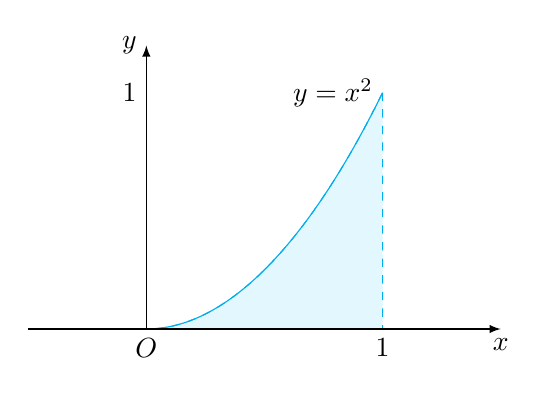
\begin{tikzpicture}[scale = 3]
            \filldraw[LightBlue] (1, 1) parabola bend (0, 0) (1, 0);
            %\draw[cyan, dashed] (1, 0) -- (1, 1);
            % \draw[cyan] (1,1) parabola bend (0,0) (1,0) -- (1,0);
            \draw[cyan, dashed] (1, 1) parabola bend (0, 0) (1,0) -- (1,1) -- cycle;
            \draw[cyan] (1, 1) parabola bend (0, 0) (1,0);
            %标注点
            \node[below] at (1,0) {$1$};
            \node[left] at (0,1) {$1$};
            \node[left] at (1, 1) {$y=x^2$};
            %标注坐标轴
            \draw[-latex] (-0.5, 0) -- (1.5, 0) node[below] {$x$};
            \draw[-latex] (0, 0) -- (0, 1.2) node[left] {$y$};
            \node[below] at (0,0) {$O$};
        \end{tikzpicture}
    \end{center}
    与之对应的概率为
    $$
        P\{X^2 \geqslant Y\}
        =\int_{-\infty}^{+\infty}\int_{-\infty}^{+\infty} f(x,y) \,\mathrm{d}x\mathrm{d}y
        = \int_{0}^{1} \mathrm{d}x \int_{0}^{x^2} \frac{1}{2}\mathrm{e}^{-\frac{y}{2}} \mathrm{d}y
        =\int_{0}^{1} 1-\mathrm{e}^{-\frac{x^2}{2}} \mathrm{d}x.
    $$
    凑出含有标准正态分布的因式
    $$
        P\{X^2 \geqslant Y\}
        = 1 - \sqrt{2\pi} \int_{0}^{1} \frac{1}{\sqrt{2\pi}} \mathrm{e}^{-\frac{x^2}{2}} \mathrm{d}x
        = 1 - \sqrt{2\pi}\left[\Phi(1)-\Phi(0)\right]
        \approx 0.1445.
    $$
    或者直接用计算器求定积分
    $$
        P\{X^2 \geqslant Y\}
        = 1 - \int_{0}^{1} \mathrm{e}^{-\frac{x^2}{2}} \mathrm{d}x
        \approx 0.1444.
    $$
\end{solution}


\begin{question}{题目24}
    设随机变量 $(X,Y)$ 的概率密度为
    $$
        f(x,y) = \begin{dcases}
            \frac{1}{2}(x+y)\mathrm{e}^{-(x+y)}, & x>0,y>0,     \\
            0,                                   & \text{其他}.
        \end{dcases}
    $$
    \begin{itemize}
        \item [(1)] 问 $X$ 和 $Y$ 是否相互独立?
        \item [(2)] 求 $Z=X+Y$ 的概率密度.
    \end{itemize}
\end{question}
\begin{solution}
    (1) 概率密度不为零的区域如图所示
    % $$
    %     G = \begin{cases}
    %         x>0, \\
    %         y>0.
    %     \end{cases}
    % $$
    \begin{center}
        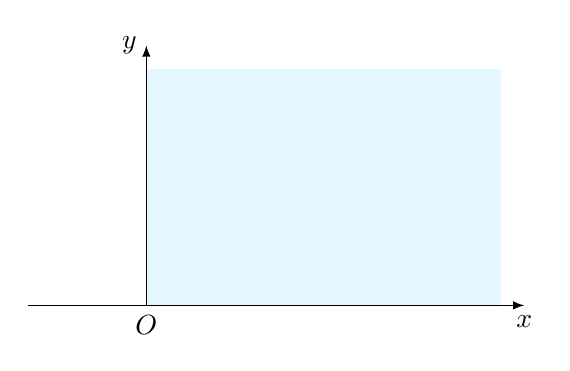
\begin{tikzpicture}[scale = 3]
            %画填充色快
            \filldraw[LightBlue] (0, 0) -- (0, 1) -- (1.5, 1) -- (1.5, 0) -- cycle;
            %标注坐标轴
            \draw[-latex] (-0.5, 0) -- (1.6, 0) node[below] {$x$};
            \draw[-latex] (0, 0) -- (0, 1.1) node[left] {$y$};
            \node[below] at (0,0) {$O$};
        \end{tikzpicture}
    \end{center}
    根据边缘概率密度的定义,$X$ 的边缘概率密度为
    $$
        \begin{aligned}
            f_X(x)
             & = \int_{-\infty}^{+\infty} f(x,y) \,\mathrm{d}y = \int_{0}^{+\infty} \frac{1}{2}(x+y)\mathrm{e}^{-(x+y)} \,\mathrm{d}y                     \\
             & = \left.-\frac{1}{2}(x+y)\mathrm{e}^{-(x+y)}\right|_{y=0}^{y=+\infty} - \int_0^{+\infty} \frac{1}{2} \mathrm{e}^{-(x+y)}\mathrm{d}[-(x+y)] \\
             & = \frac{x}{2}\mathrm{e}^{-x} - \left.\left[\frac{1}{2}\mathrm{e}^{-(x+y)}\right]\right|_{y=0}^{y=+\infty}                                  \\
             & = \frac{x}{2}\mathrm{e}^{-x} + \frac{1}{2}\mathrm{e}^{-x}.
        \end{aligned}
    $$
    即
    $$
        f_X(x) = \begin{dcases}
            \frac{\mathrm{e}^{-x}}{2}(x+1), & x>0,         \\
            0,                              & \text{其他}.
        \end{dcases}
    $$
    同理,$Y$ 的边缘概率密度为
    $$
        f_Y(y) = \int_{-\infty}^{+\infty} f(x,y) \,\mathrm{d}x
        = \begin{dcases}
            \frac{\mathrm{e}^{-y}}{2}(y+1), & y>0,         \\
            0,                              & \text{其他}.
        \end{dcases}
    $$
    由此可知
    $$
        f_X(x)f_Y(y) \neq f(x,y).
    $$
    即 $X$ 和 $Y$ 不独立.\\
    (2) 概率密度不为零的区域如图所示
    \begin{center}
        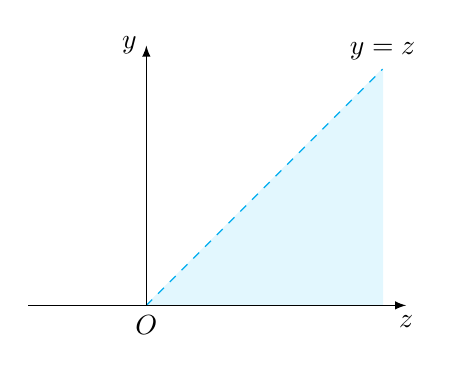
\begin{tikzpicture}[scale = 3]
            %画填充色快
            \filldraw[LightBlue] (0, 0) -- (1, 0) -- (1, 1) -- cycle;
            \draw[cyan, dashed] (0, 0) -- (1, 1);
            %画坐标系并标注
            \draw[-latex] (-0.5, 0) -- (1.1, 0) node[below] {$z$};
            \draw[-latex] (0, 0) -- (0, 1.1) node[left] {$y$};
            \node[below] at (0, 0) {$O$};
            %标注区域边界
            \node[above] at (1,1) {$y=z$};
        \end{tikzpicture}
    \end{center}
    根据两个随机变量的函数分布,$Z=X+Y$ 的概率密度可表示为
    $$
        f_Z(z) = \int_{-\infty}^{+\infty} f(z-y,y) \,\mathrm{d}y
        = \int_0^z\frac{1}{2}(z-y+y)\mathrm{e}^{-(z-y+y)}\mathrm{d}y
        %& = \begin{dcases} \frac{1}{2} \int_0^z z\mathrm{e}^{-z} \mathrm{d}y, & z-y>0, y>0, \\ 0,& \text{其他}. \end{dcases}
        = \begin{dcases}
            \frac{z^2}{2}\mathrm{e}^{-z}, & z>0,z>y      \\
            0,                            & \text{其他}.
        \end{dcases}
    $$
\end{solution}


\section{随机变量的数字特征}

\begin{comment}
\begin{question}{例题5}
    设随机变量 $X$ 服从瑞利分布,即其概率密度为
    $$
        f(x) = \begin{dcases}
            \frac{x}{\sigma^2} \mathrm{e}^{-\frac{x^2}{2\sigma^2}}, & x>0,           \\
            0,                                                      & x \leqslant 0.
        \end{dcases}
    $$
    其中 $\sigma>0$ 是常数,求 $E(X), D(X)$.
\end{question}
\begin{solution}
    根据概率密度的定义,其数学期望为
    $$
        E(X) = \int_{-\infty}^{+\infty} xf(x) \ \mathrm{d}x
        = \int_{0}^{+\infty} \frac{x^2}{\sigma^2} \mathrm{e}^{-\frac{x^2}{2\sigma^2}} \ \mathrm{d}x
        = \sqrt{\frac{\pi}{2}}\sigma
    $$
    根据方差的性质
    $$
        \begin{aligned}
            D(X)
             & = E\left(X^2\right) - E^2(X)                                                                                       \\
             & = \int_0^{+\infty} x^2 f(x) \,\mathrm{d}x - \left(\sqrt{\frac{\pi}{2}}\sigma\right)^2                              \\
             & = \int_0^{+\infty} x^2\frac{x}{\sigma^2} \mathrm{e}^{-\frac{x^2}{2\sigma^2}} \,\mathrm{d}x - \frac{\pi}{2}\sigma^2 \\
             & = 2\sigma^2\int_0^{+\infty}\frac{x^2}{2\sigma^2}
            \mathrm{e}^{-\frac{x^2}{2\sigma^2}} \,\mathrm{d}\left(\frac{x^2}{2\sigma^2}\right) - \frac{\pi}{2}\sigma^2            \\
        \end{aligned}
    $$
    令 $\dfrac{x^2}{2\sigma^2} > 0$ 有
    $$
        D(X) = 2\sigma^2\int_0^{+\infty}t \mathrm{e}^{-t} \,\mathrm{d}t - \frac{\pi}{2}\sigma^2 = 2\sigma^2 - \frac{\pi}{2}\sigma^2
    $$
\end{solution}
\end{comment}


\begin{question}{题目2}
    某产品的次品率为 0.1,检验员每天检验 4 次. 每次随机地取 10 件产品进行检验,如发现其中的次品数多于 1,就去调整设备. 以 $X$ 表示一天中调整设备的次数,试求 $E(X)$. (设诸产品是否为次品是相互独立的.)
\end{question}
\begin{solution}
    抽检时次品数多于 1 ,即需要调整设备的概率为
    $$
        \begin{aligned}
            p & = 1 - C_{10}^{0}(0.1)^0(1-0.1)^{10} - C_{10}^{1}(0.1)^1(1-0.1)^9 \\
              & = 1 - (0.9)^{10} - (0.9)^9                                       \\
              & \approx 0.2639.                                                  \\
        \end{aligned}
    $$
    调整设备的次数 $X$ 所服从的分布律为
    $$
        p_k = C_4^k p^k (1-p)^{4-k}.
    $$
    $$
        \begin{array}{c|ccccc}
            X   & 0       & 1         & 2           & 3         & 4   \\
            \hline
            p_k & (1-p)^4 & 4p(1-p)^3 & 6p^2(1-p)^2 & 4p^3(1-p) & p^4
        \end{array}
    $$
    其数学期望为
    $$
        E(X) = \sum_{k=0}^{4} p_kX_k
        = 0 + 4p(1-p)^3 + 12p^2(1-p)^2 + 12p^3(1-p) + 4p^4
        \approx 1.0556.
    $$
\end{solution}



\begin{question}{题目4}
    \begin{enumerate}
        \item [(1)] 设随机变量 $X$ 的分布律为 $\displaystyle P\left\{X=(-1)^{j+1}\frac{3^j}{j}\right\} = \frac{2}{3^j}, j = 1, 2, \cdots $,说明 $X$ 的数学期望不存在.
        \item [(2)]  一盒中装有一只黑球,一只白球,作摸球游戏,规则如下:一次从盒中随机摸一只球,若摸到白球,则游戏结束,摸到黑球放回再放入一只黑球,然后再从盒中随机地摸一只球. 试说明要游戏结束的摸球次数 $X$ 的数学期望不存在.
    \end{enumerate}
\end{question}
\begin{solution}
    (1) 根据数学期望的定义
    $$
        E(X) = \sum_{k=1}^{\infty} x_kp_k
        = \sum_{k=1}^{\infty} (-1)^{k+1} \frac{3^k}{k} \cdot \frac{2}{3^k}
        = 2\sum_{k=1}^{\infty} \frac{(-1)^{k+1}}{k}
        < 2\sum_{k=1}^{\infty} \left|\frac{1}{k}\right|.
    $$
    根据判断调和级数敛散性的积分放缩法
    \begin{center}
        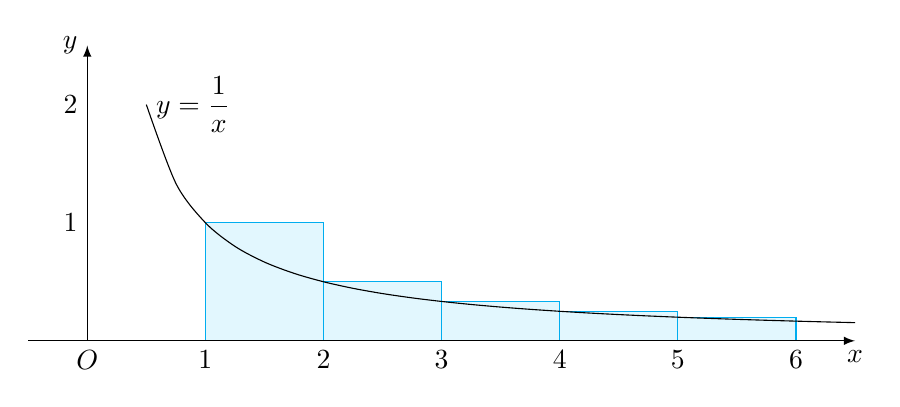
\begin{tikzpicture}[scale = 1.5]
            %画一系列方块
            \filldraw[LightBlue] (1, 0) -- (1, 1) -- (2, 1) -- (2, 0);
            \draw[cyan] (1, 0) -- (1, 1) -- (2, 1) -- (2, 0);
            \filldraw[LightBlue] (2, 0) -- (2, 0.5) -- (3, 0.5) -- (3, 0);
            \draw[cyan] (2, 0) -- (2, 0.5) -- (3, 0.5) -- (3, 0);
            \filldraw[LightBlue] (3, 0) -- (3, 1/3) -- (4, 1/3) -- (4, 0);
            \draw[cyan] (3, 0) -- (3, 1/3) -- (4, 1/3) -- (4, 0);
            \filldraw[LightBlue] (4, 0) -- (4, 0.25) -- (5, 0.25) -- (5, 0);
            \draw[cyan] (4, 0) -- (4, 0.25) -- (5, 0.25) -- (5, 0);
            \filldraw[LightBlue] (5, 0) -- (5, 0.2) -- (6, 0.2) -- (6, 0);
            \draw[cyan] (5, 0) -- (5, 0.2) -- (6, 0.2) -- (6, 0);

            %标注x轴上的点
            \node[below] at (1, 0) {$1$};
            \node[below] at (2, 0) {$2$};
            \node[below] at (3, 0) {$3$};
            \node[below] at (4, 0) {$4$};
            \node[below] at (5, 0) {$5$};
            \node[below] at (6, 0) {$6$};

            %标注y轴上的点
            \node[left] at (0, 1) {$1$};
            \node[left] at (0, 2) {$2$};

            %画函数图像
            \draw[domain = 0.5 : 6.5, smooth] plot(\x, {1/\x});
            \node[right] at (0.5, 2) {$y = \dfrac{1}{x}$};

            %画坐标轴,坐标轴覆盖在最上层
            \draw[-latex] (-0.5, 0) -- (6.5, 0) node[below] {$x$};
            \draw[-latex] (0, 0) -- (0, 2.5) node[left] {$y$};
            \node[below]  at (0,0) {$O$};
        \end{tikzpicture}
    \end{center}
    $$
        \sum_{k=1}^{\infty}\frac{1}{k} > \int_{1}^{+\infty}\frac{1}{x}\,\mathrm{d}x \to \infty.
    $$
    这说明调和级数 $\displaystyle \sum_{k=1}^{\infty} \frac{1}{k}$ 不绝对收敛,级数 $\displaystyle 2\sum_{k=1}^{\infty} \frac{(-1)^{k+1}}{k}$ 也不绝对收敛,所以 $X$ 的数学期望不存在.
    \begin{comment}
    (2) 摸球次数 $X$ 应当满足如下规律
    $$
        \renewcommand\arraystretch{2}
        \setlength{\arraycolsep}{24mm}
        \begin{array}{c|c}
            \hline
            \text{摸球次数} & \text{概率}                                                 \\
            \hline
            1           & P\{X=1\} = \dfrac{1}{2}                                   \\
            2           & P\{X=2\} = \dfrac{1}{2}\cdot\dfrac{1}{3}                  \\
            3           & P\{X=3\} = \dfrac{1}{2}\cdot\dfrac{1}{3}\cdot\dfrac{1}{4} \\
            \vdots      & \vdots                                                    \\
            n           & \displaystyle P\{X=n\} = \prod_{k=1}^{n+1}\frac{1}{k}     \\
            \vdots      & \vdots                                                    \\
            \hline
        \end{array}
    $$
    数学期望 $E(X)$ 为
    $$
        E(X) = \sum_{k=1}^{\infty} x_kp_k
        = \sum_{k=1}^{\infty}\frac{k}{2+(k-1)}
        = \sum_{k=1}^{\infty} 1 - \frac{1}{k-1}
        =
    $$
    \end{comment}

\end{solution}

\begin{question}{题目14}
    设随机变量 $X_1, X_2$ 的概率密度分别为
    $$
        f_1(x) = \begin{cases}
            2\mathrm{e}^{-2x}, & x > 0,         \\
            0,                 & x \leqslant 0.
        \end{cases}
        \quad
        f_2(x) = \begin{cases}
            4\mathrm{e}^{-4x}, & x > 0,         \\
            0,                 & x \leqslant 0.
        \end{cases}
    $$
    \begin{enumerate}
        \item[(1)] 求 $E(X_1 + X_2), E\left(2X_1 - 3X_2^2\right)$.
        \item[(2)] 又设 $X_1,X_2$ 相互独立,求 $E(X_1X_2)$.
    \end{enumerate}
\end{question}
\begin{solution}
    如果随机变量 $X$ 服从参数为 $\theta$ 的指数分布,那么其数学期望为
    \begin{equation}\label{指数分布的均值}
        \begin{aligned}
            E(X)
             & = \int_{-\infty}^{+\infty} xf(x) \,\mathrm{d}x = \int_{0}^{+\infty} \frac{x}{\theta}\mathrm{e}^{-\frac{x}{\theta}} \mathrm{d}x \\
            %& = \int_{0}^{+\infty} -x \,\mathrm{d}\left(\mathrm{e}^{-\frac{x}{\theta}}\right)                                                \\
             & = -x\mathrm{e}^{-\frac{x}{\theta}}\Big|_{0}^{+\infty} - \int_{0}^{+\infty} \mathrm{e}^{-\frac{x}{\theta}} \mathrm{d}(-x)       \\
             & = 0 - \theta\mathrm{e}^{-\frac{x}{\theta}}\Big|_{0}^{+\infty}                                                                  \\
             & = \theta.
        \end{aligned}
    \end{equation}
    类似地,$X^2$ 的数学期望为
    \begin{equation}
        \begin{aligned}
            E(X^2)
             & = \int_{-\infty}^{+\infty} x^2f(x) \,\mathrm{d}x
            = \int_{0}^{+\infty} \frac{x^2}{\theta}\mathrm{e}^{-\frac{x}{\theta}} \mathrm{d}x                                                \\
             & = -x^2\mathrm{e}^{-\frac{x}{\theta}}\Big|_{0}^{\infty} - \int_{0}^{+\infty} \mathrm{e}^{-\frac{x}{\theta}} \,\mathrm{d}(-x^2) \\
             & = 0 + \int_{0}^{+\infty} 2x\mathrm{e}^{-\frac{x}{\theta}} \,\mathrm{d}x                                                       \\
             & = 2\theta\int_{0}^{+\infty} \frac{x}{\theta}\mathrm{e}^{-\frac{x}{\theta}} \,\mathrm{d}x,                                     \\
        \end{aligned}
    \end{equation}
    根据式 $\eqref{指数分布的均值}$ 中已经证明的结论
    \begin{equation}
        E(X^2) = 2\theta \cdot \theta = 2\theta^2.
    \end{equation}
    根据方差的性质
    \begin{equation}\label{指数分布的方差}
        D(X) = E(X^2) - E^2(X) = 2\theta^2 - \theta^2 = \theta^2.
    \end{equation}
    (1) 考虑到 $X_1 \sim E\left(\dfrac{1}{2}\right), X_2 \sim E\left(\dfrac{1}{4}\right)$
    $$
        E(X_1+X_2) = E(X_1) + E(X_2) = \frac{1}{2} + \frac{1}{4} = \frac{3}{4}.
    $$
    $$
        E\left(2X_1 - 3X_2^2\right)
        = 2E(X_1) - 3E(X_2^2)
        = 2\cdot\frac{1}{2} - 3 \cdot 2\left(\frac{1}{4}\right)^2
        = \frac{5}{8}.
    $$
    (2) 如果$X_1,X_2$ 相互独立,那么
    $$
        E(X_1X_2) = E(X_1)E(X_2) = \frac{1}{2} \cdot \frac{1}{4} = \frac{1}{8}.
    $$
\end{solution}


\begin{question}{题目22}
    设随机变量 $X_1, X_2, X_3, X_4$ 相互独立,且有 $E(X_i)=i$,$D(X) = 5-i$,$i = 1, 2, 3, 4$. 设 $Y = 2X_1 - X_2 + 3X_3 - \dfrac{1}{2}X_4$,求 $E(Y), D(Y)$.
\end{question}
\begin{solution}
    根据数学期望的性质
    $$
        \begin{aligned}
            E(Y)
             & = E\left(2X_1 - X_2 + 3X_3 - \frac{1}{2}X_4\right) \\
             & = 2E(X_1) - E(X_2) + 3E(X_3) - \frac{1}{2}E(X_4)   \\
             & = 2 - 2 + 3 \times 3 - \frac{1}{2} \times 4        \\
             & = 7.                                               \\
        \end{aligned}
    $$
    根据方差的性质
    $$
        \begin{aligned}
            D(Y)
             & = D\left(2X_1 - X_2 + 3X_3 - \frac{1}{2}X_4\right)   \\
             & = 4D(X_1) + D(X_2) + 9D(X_3) + \frac{1}{4}D(X_4)     \\
             & = 4 \times 4 + 3 + 9 \times 2 + \frac{1}{4} \times 1 \\
             & = \frac{149}{4}.
        \end{aligned}
    $$
\end{solution}



\begin{question}{题目32}
    设随机变量 $(X,Y)$ 具有概率密度
    $$
        f(x,y) = \begin{dcases}
            \frac{1}{8}(x+y), & 0 \leqslant x \leqslant 2, 0 \leqslant y \leqslant 2, \\
            0,                & \text{其他}.
        \end{dcases}
    $$
    求 $E(X), E(Y), \cov(X,Y), \rho_{XY}, D(X+Y)$.
\end{question}
\begin{solution}
    概率密度不为零的区域如图所示
    \begin{center}
        \begin{center}
            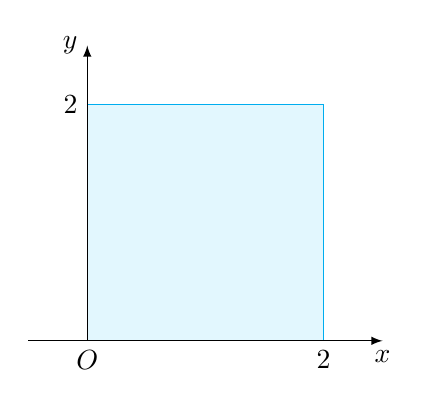
\begin{tikzpicture}[scale = 1.5]
                %画填充色快
                \filldraw[LightBlue] (0, 0) -- (2, 0) -- (2, 2) -- (0,2) -- cycle;
                \draw[cyan] (0, 0) -- (2, 0) -- (2, 2) -- (0,2) -- cycle;
                %画坐标系并标注
                \draw[-latex] (-0.5, 0) -- (2.5, 0) node[below] {$x$};
                \draw[-latex] (0, 0) -- (0, 2.5) node[left] {$y$};
                \node[below] at (0, 0) {$O$};
                %标注区域边界
                \node[below] at (2, 0) {$2$};
                \node[left] at (0, 2) {$2$};
            \end{tikzpicture}
        \end{center}
    \end{center}
    根据数学期望的定义,$X$ 的数学期望为
    $$
        \begin{aligned}
            E(X)
             & = \int_{-\infty}^{+\infty}\int_{-\infty}^{+\infty} xf(x,y) \,\mathrm{d}x\mathrm{d}y
            = \int_0^2 \mathrm{d}x\int_0^2\frac{x}{8}(x+y)\,\mathrm{d}y                                                 \\
             & = \int_0^2 \left.\left(\frac{x^2}{8}y + \frac{x}{8}\frac{y^2}{2}\right)\right|_{y=0}^{y=2} \,\mathrm{d}x
            = \int_0^2 \frac{x^2}{4} + \frac{x}{4} \,\mathrm{d}x                                                        \\
             & =\left.\left(\frac{x^3}{12} + \frac{x^2}{8}\right)\right|_{x=0}^{x=2}  = \frac{7}{6} .                   \\
        \end{aligned}
    $$
    $X^2$ 的数学期望为
    $$
        \begin{aligned}
            E(X^2)
             & = \int_{-\infty}^{+\infty}\int_{-\infty}^{+\infty} x^2f(x,y) \,\mathrm{d}x\mathrm{d}y
            = \int_0^2 \mathrm{d}x\int_0^2\frac{x^2}{8}(x+y)\,\mathrm{d}y                                                 \\
             & = \int_0^2 \left.\left(\frac{x^3}{8}y + \frac{x^2}{8}\frac{y^2}{2}\right)\right|_{y=0}^{y=2} \,\mathrm{d}x
            = \int_0^2 \frac{x^3}{4} + \frac{x^2}{4} \,\mathrm{d}x                                                        \\
             & = \left.\left(\frac{x^4}{16} + \frac{x^3}{12}\right)\right|_{x=0}^{x=2}  = \frac{5}{3}.                    \\
        \end{aligned}
    $$
    $XY$ 的数学期望为
    $$
        \begin{aligned}
            E(XY)
             & = \int_{-\infty}^{+\infty}\int_{-\infty}^{+\infty} xyf(x,y) \,\mathrm{d}x\mathrm{d}y = \int_0^2 \mathrm{d}x\int_0^2\frac{xy}{8}(x+y)\,\mathrm{d}y                      \\
             & = \int_0^2 \left.\left(\frac{x^2}{8}\frac{y^2}{2} + \frac{x}{8}\frac{y^3}{3}\right)\right|_{y=0}^{y=2}\mathrm{d}x = \int_0^2 \frac{x^2}{4} + \frac{x}{3} \,\mathrm{d}x \\
             & = \left.\left(\frac{x^3}{12} + \frac{x^2}{6}\right)\right|_{x=0}^{x=2}   = \frac{4}{3}.                                                                                \\
        \end{aligned}
    $$
    同理
    $$
        E(Y) = \frac{7}{6}, \quad E(Y^2) = \frac{5}{3}.
    $$
    根据数学期望的性质
    $$
        D(X)
        = E\left\{[X - E(X)]^2\right\}
        = E(X^2)-E^2(X)
        = \frac{5}{3}-\left(\frac{7}{6}\right)^2
        = \frac{11}{36}.
    $$
    $$
        D(Y)
        = E\left\{[Y - E(Y)]^2\right\}
        = E(Y^2)-E^2(Y)
        = \frac{5}{3}-\left(\frac{7}{6}\right)^2
        = \frac{11}{36}.
    $$
    根据协方差的定义
    $$
        \cov(X,Y)
        = E\{[X-E(X)][Y-E(Y)]\}
        = E(XY) - E(X)E(Y)
        = \frac{4}{3} - \frac{7}{6} \times \frac{7}{6}
        = -\frac{1}{36}.
    $$
    根据相关系数的定义和方差的性质
    $$
        \rho_{XY}
        = \frac{\cov(X,Y)}{\sqrt{D(X)}\sqrt{D(Y)}}
        = \frac{-\frac{1}{36}}{\sqrt{\frac{11}{36}}\sqrt{\frac{11}{36}}}
        = -\frac{1}{11}.
    $$
    根据方差的性质
    $$
        \begin{aligned}
            D(X+Y)
             & = E\left\{[(X+Y) - E(X+Y)]^2\right\}                                                          \\
             & = E\left\{[(X-E(X)) + (Y-E(Y))]^2\right\}                                                     \\
             & = E\left\{[X-E(X)]^2\right\} + E\left\{[Y-E(Y)]^2\right\} + 2E\left\{[X-E(X)][Y-E(Y)]\right\} \\
             & = D(X) + D(Y) + 2\cov(X,Y)                                                                    \\
             & = \frac{11}{36} + \frac{11}{36} + 2 \times \left(-\frac{1}{36}\right)                         \\
             & = \frac{5}{9}.
        \end{aligned}
    $$
\end{solution}



\begin{question}{题目33}
    设随机变量 $X \sim N(\mu, \sigma^2)$,$Y \sim N(\mu, \sigma^2)$,且设 $X,Y$ 相互独立,试求 $Z_1 = \alpha X + \beta Y$ 和 $Z_2 = \alpha X - \beta Y$ 的相关系数(其中 $\alpha, \beta$ 是不为零的常数).
\end{question}
\begin{solution}
    根据协方差的定义和数学期望的性质,结合 $X,Y$ 的独立性
    $$
        \begin{aligned}
            \cov(Z_1, Z_2)
            %& = E\left\{[Z_1-E(Z_1)][Z_2-E(Z_2)]\right\}                               \\
             & = E(Z_1Z_2) - E(Z_1)E(Z_2)                                                              \\
             & = E(\alpha^2X^2-\beta^2Y^2) - E(\alpha X + \beta Y)E(\alpha X - \beta Y)                \\
             & = \alpha^2E(X^2) - \beta^2E(Y^2) - [\alpha E(X) + \beta E(Y)][\alpha E(X) - \beta E(Y)] \\
             & = \alpha^2[E(X^2)-E^2(X)] - \beta^2 [E(Y^2)-E^2(Y)]                                     \\
             & = (\alpha^2 - \beta^2)\sigma^2.                                                         \\
        \end{aligned}
    $$
    根据方差的性质
    $$
        D(Z_1) = D(\alpha X + \beta Y)
        = \alpha^2D(X) + \beta^2D(Y)
        = (\alpha^2+\beta^2)\sigma^2.
    $$
    $$
        D(Z_2) = D(\alpha X - \beta Y)
        = \alpha^2D(X) + \beta^2D(Y)
        = (\alpha^2+\beta^2)\sigma^2.
    $$
    相关系数为
    $$
        \rho_{Z_1Z_2} = \frac{\cov(Z_1, Z_2)}{\sqrt{D(Z_1)}\sqrt{D(Z_2)}}
        = \frac{(\alpha^2 - \beta^2)\sigma^2}{\sqrt{(\alpha^2+\beta^2)\sigma^2}\sqrt{(\alpha^2+\beta^2)\sigma^2}}
        = \frac{\alpha^2-\beta^2}{\alpha^2+\beta^2}.
    $$
\end{solution}
\section{样本及抽样分布}


\begin{question}{题目1}
    在总体 $N(52, 6.3^2)$ 中随机抽取一容量为 36 的样本,求样本均值落在 $50.8$ 到 $53.8$ 之间的概率.
\end{question}
\begin{solution}
    根据正态总体的样本均值与样本方差的分布
    $$
        \overline{X} \sim N\left(\mu, \frac{\sigma^2}{n}\right) = N(52, 1.05^2).
    $$
    从而有
    $$
        \begin{aligned}
            P\left\{50.8 < \overline{X} < 53.8\right\}
             & = P\left\{\frac{50.8-52}{1.05} < \frac{\overline{X}-52}{1.05} < \frac{53.8-52}{1.05} \right\} \\
             & = P\left\{-\frac{8}{7} < \frac{\overline{X}-52}{1.05} < \frac{12}{7} \right\}                 \\
             & = \Phi\left(\frac{12}{7}\right) - \Phi\left(-\frac{8}{7}\right)                               \\
             & = 0.8302.
        \end{aligned}
    $$
\end{solution}


\begin{question}{题目2}
    在总体 $N(12, 4)$ 中随机抽一容量为 5 的样本 $X_1, X_2, X_3, X_4, X_5$.
    \begin{enumerate}
        \item [(1)] 求样本均值与总体均值之差的绝对值大于 1 的概率.
        \item [(2)] 求概率 $P\{\max\{X_1, X_2, X_3, X_4, X_5\} > 15\}$,$P\{\min\{X_1, X_2, X_3, X_4, X_5\} < 10\}$.
    \end{enumerate}
\end{question}
\begin{solution}
    (1) 由于样本 $X_1, X_2, X_3, X_4, X_5$ 来自正态总体,所以
    $$
        \overline{X} \sim N\left(\mu, \frac{\sigma^2}{n}\right) = N\left(12, 0.8\right).
    $$
    样本均值与总体均值之差的绝对值大于 1 的概率
    $$
        \begin{aligned}
            P\{|\overline{X} - \mu| > 1\}
             & = 1 - P\{\overline{X} - \mu \leqslant 1 \}                                                                                 \\
             & = 1 - P\{-1 \leqslant \overline{X}-12 \leqslant 1\}                                                                        \\
             & = 1 - P\left\{ -\frac{1}{\sqrt{0.8}} \leqslant \frac{\overline{X} - 12}{\sqrt{0.8}} \leqslant \frac{1}{\sqrt{0.8}}\right\} \\
             & = 1 - \left[\Phi\left(\frac{1}{\sqrt{0.8}}\right) - \Phi\left(-\frac{1}{\sqrt{0.8}}\right)\right]                          \\
             & = 0.2636.
        \end{aligned}
    $$
    (2) 因 $X_i$ 的分布函数为 $\Phi\left(\dfrac{x-12}{2}\right)$,故 $M = \max\{X_1, X_2, X_3, X_4, X_5\}$ 的分布函数为
    $$
        F_M(x) = \left[\Phi\left(\frac{x-12}{2}\right)\right]^5,
    $$
    因此
    $$
        \begin{aligned}
            P\{\max\{X_1, X_2, X_3, X_4, X_5\} > 15\}
             & = P\{M > 15\}                                         \\
             & = 1 - P\{M>15\}                                       \\
             & = 1 - F_M(15)                                         \\
             & = 1 - \left[\Phi\left(\frac{15-12}{2}\right)\right]^5 \\
             & = 0.2923.
        \end{aligned}
    $$
    记$N = \min\{X_1, X_2, X_3, X_4, X_5\}$,则 $N$ 的分布函数为
    $$
        F_N(x) = 1 - \left[1-\Phi\left(\frac{x-12}{2}\right)\right]^5,
    $$
    因此
    $$
        \begin{aligned}
            P\{\min\{X_1, X_2, X_3, X_4, X_5\} < 10\}
             & = P\{N<10\}                                               \\
             & = 1 - \left[1 - \Phi\left(\frac{10-12}{2}\right)\right]^5 \\
             & = 1 - [1-\Phi(-1)]^5                                      \\
             & = 1 - \Phi(1)^5                                           \\
             & = 0.5785.
        \end{aligned}
    $$
\end{solution}






\begin{question}{题目4}
    \begin{enumerate}
        \item [(1)] 设样本 $X_1, X_2, \cdots, X_6$ 来自总体 $N(0,1)$ ,$Y=(X_1+X_2+X_3)^2 + (X_4+X_5+X_6)^2$ ,试确定常数 $C$ 使 $CY$ 服从 $\chi^2$ 分布.
        \item [(2)] 设样本 $X_1, X_2, \cdots, X_5$ 来自总体 $N(0,1)$ ,$Y = \dfrac{C(X_1+X_2)}{\sqrt{X_3^2 + X_4^2 + X_5^2}}$ ,试确定常数 $C$ 使 $Y$ 服从 $t$ 分布.
              %\item [(3)] 已知 $X \sim t(n)$ ,求证 $X^2 \sim F(1,n)$.
    \end{enumerate}
\end{question}
\begin{solution}
    (1) 因为样本来自正态总体 $N(0,1)$,所以
    $$
        X_1 + X_2 + X_3 \sim N(0, 3), \quad
        X_4 + X_5 + X_6 \sim N(0, 3),
    $$
    将二者都化为标准正态分布
    $$
        \frac{X_1 + X_2 + X_3}{\sqrt{3}} \sim N(0, 1), \quad
        \frac{X_4 + X_5 + X_6}{\sqrt{3}} \sim N(0, 1),
    $$
    由于样本间彼此独立,所以根据 $\chi^2$ 分布的定义,有
    $$
        \left(\frac{X_1 + X_2 + X_3}{\sqrt{3}}\right)^2 + \left(\frac{X_4 + X_5 + X_6}{\sqrt{3}}\right)^2 \sim \chi^2(2),
    $$
    与 $Y$ 对比系数,得到
    $$
        C = \frac{1}{3}.
    $$
    (2) 考虑到 $X_1, X_2, \cdots, X_n$ 是总体 $N(0,1)$ 的样本,所以
    $$
        X_1 + X_2 \sim N(0,2), \quad \frac{X_1 + X_2}{\sqrt{2}} \sim N(0,1),
    $$
    另一方面
    $$
        X_3^2 + X_4^2 + X_5^2 \sim \chi^2(3),
    $$
    结合 $\dfrac{X_1 + X_2}{\sqrt{2}}$ 与 $X_3^2 + X_4^2 + X_5^2$ 的独立性
    $$
        \frac{\dfrac{X_1+X_2}{\sqrt{2}}}{\sqrt{(X_3^2 + X_4^2 + X_5^2)/3}}
        = \sqrt{\frac{3}{2}} \frac{X_1+X_2}{\sqrt{X_3^2 + X_4^2 + X_5^2}}
        \sim t(3),
    $$
    综上
    $$
        C = \sqrt{\frac{3}{2}}.
    $$
\end{solution}





\begin{question}{题目6}
    设总体 $X \sim b(1,p)$,$X_1, X_2, \cdots X_n$ 是来自 $X$ 的样本.
    \begin{enumerate}
        \item [(1)] 求 $(X_1, X_2, \cdots, X_n)$ 的分布律.
        \item [(2)] 求 $\displaystyle \sum_{i=1}^{n} X_i$ 的分布律.
        \item [(3)] 求 $E(\overline{X}), D(\overline{X}), E(S^2)$.
    \end{enumerate}
\end{question}
\begin{solution}
    (1) 由于样本 $X_i \sim b(1,p)$,所以
    $$
        P\{X_i = x_i\} = p^{x_i}(1-p)^{1-x_i} (x_i = 0, 1).
    $$
    又因为样本间彼此独立,所以
    $$
        \begin{aligned}
            P\{X_1, X_2, \cdots, X_n\}
             & = P\{X_1 = x_1\} \cdot P\{X_2 = x_2\} \cdots P\{X_n = x_n\}                   \\
             & = p^{x_1}(1-p)^{1-x_1} \cdot p^{x_2}(1-p)^{1-x_2} \cdots p^{x_n}(1-p)^{1-x_n} \\
             & = \prod_{i=1}^{n} p^{x_i}(1-p)^{1-x_i}                                        \\
             & = p^{\sum_{i=1}^{n} x_i}(1-p)^{\sum_{i=1}^{n} 1-x_i}.                         \\
        \end{aligned}
    $$
    (2) 由于样本 $X_i \sim b(1,p)$ 且彼此相互独立,这显然满足二项分布的定义,所以
    $$
        \sum_{i=1}^{n} X_i \sim b(n,p)
    $$
    其分布律为
    $$
        P\left\{\sum_{i=1}^n X_i = k\right\}
        = C_n^k p^k (1-p)^{n-k}
    $$
    (3) 由于总体 $X \sim b(1,p)$,$E(X) = p$,$D(X) = p(1-p)$,所以
    $$
        E(\overline{X}) = \mu = p,
    $$
    $$
        D(\overline{X}) = \frac{\sigma^2}{n} = \frac{p(1-p)}{n},
    $$
    $$
        E(S^2) = \sigma^2 = p(1-p).
    $$
\end{solution}
\section{参数估计}

\begin{question}{题目4}
    \begin{enumerate}
        \item [(1)] 设总体 $X$ 具有分布律
              $$
                  \begin{array}{c|ccc}
                      X   & 1        & 2                 & 3            \\
                      \hline
                      p_k & \theta^2 & 2\theta(1-\theta) & (1-\theta)^2
                  \end{array}
              $$
              其中 $\theta(0 < \theta < 1)$ 为未知参数. 已知取得了样本值 $x_1 = 1, x_2 = 2, x_3 = 1$. 试求 $\theta$ 的矩估计值和最大似然估计值.
    \end{enumerate}
\end{question}
\begin{solution}
    (1) 对于矩估计值
    $$
        \mu_1 = E(X) = \sum_{k=1}^{\infty} x_kp_k = \theta^2+4\theta(1-\theta)+3(1-\theta)^2,
    $$
    解得
    $$
        \theta = \frac{1}{2}(3-\mu_1),
    $$
    所以 $\theta$ 的估计量为
    $$
        \hat{\theta} = \frac{1}{2}(3-\overline{x}) = \frac{5}{6}.
    $$
    对于最大似然估计值
    $$
        L(\theta) = \prod_{i=1}^{3} P\{X_i = x_i\}
        = \theta^2 \cdot 2\theta(1-\theta) \cdot \theta^2
        = 2\theta^5(1-\theta),
    $$
    两边取对数
    $$
        \ln L(\theta) = \ln2 + 5\ln\theta + \ln(1-\theta),
    $$
    两边求导,令导函数为零
    $$
        \ln L'(\theta) = \frac{5}{\theta} - \frac{1}{1-\theta} = 0,
    $$
    所以 $\theta$ 的最大似然估计值为
    $$
        \hat{\theta} = \frac{5}{6}.
    $$
\end{solution}



\begin{question}{题目5(2)}
    设某种电子器件的寿命 (以h计)$T$ 服从双参数的指数分布,其概率密度为
    $$
        f(t) = \begin{dcases}
            \frac{1}{\theta}\mathrm{e}^{-\frac{t-c}{\theta}}, & t \geqslant c, \\
            0,                                                & \text{其他}.
        \end{dcases}
    $$
    其中 $c,\theta(c,\theta > 0)$ 为未知参数. 自一批这种器件中随机地取 $n$ 件进行寿命试验. 设它们的失效时间依次为 $x_1 \leqslant x_2 \leqslant \cdots \leqslant x_n$.
    \begin{enumerate}
        \item [(1)] 求 $\theta$ 与 $c$ 的最大似然估计值.
        \item [(2)] 求 $\theta$ 与 $c$ 的矩估计值.
    \end{enumerate}
\end{question}
\begin{solution}
    (2) 对于矩估计值
    $$
        \mu_l = \int_{-\infty}^{+\infty} t^l f(t) \,\mathrm{d}t
        = \int_{c}^{+\infty} \frac{t^l}{\theta}\mathrm{e}^{-\frac{t-c}{\theta}} \,\mathrm{d}t,
    $$
    令 $x = \dfrac{t-c}{\theta}$ 有
    $$
        \mu_1 = \int_0^{+\infty} \frac{\theta x + c}{\theta} \mathrm{e}^{-x} \,\mathrm{d}(\theta x + c)
        = \int_0^{+\infty} (\theta x + c) \mathrm{e}^{-x} \,\mathrm{d}x
        = \theta + c,
    $$
    $$
        \mu_2 = \int_0^{+\infty} \frac{(\theta x + c)^2}{\theta} \mathrm{e}^{-x} \,\mathrm{d}(\theta x + c)
        = \int_0^{+\infty} \left(\theta^2x^2 + 2\theta cx + c^2\right)\mathrm{e}^{-x} \,\mathrm{d}x
        = 2\theta^2 + 2\theta c + c^2.
    $$
    反解得到
    $$
        \begin{cases}
            \theta = \sqrt{\mu_2 - \mu_1^2}         \\
            c      = \mu_1 - \sqrt{\mu_2 - \mu_1^2} \\
        \end{cases}
    $$
    带入样本数据,有
    $$
        \hat{\theta} = \sqrt{\frac{1}{n}\sum_{i=1}^n(X_i-\overline{X})^2}
    $$
    $$
        \hat{c} = \overline{X} - \sqrt{\frac{1}{n}\sum_{i=1}^n(X_i-\overline{X})^2}
    $$
\end{solution}



\begin{question}{题目8}
    \begin{enumerate}
        \item [(1)] 设 $X_1, X_2, \cdots, X_n$ 是来自概率密度为
              $$
                  f(x; \theta) = \begin{dcases}
                      \theta x^{\theta - 1}, & 0<x<1,       \\
                      0,                     & \text{其他}.
                  \end{dcases}
              $$
              的总体的样本,$\theta$ 未知,求 $U = \mathrm{e}^{-\frac{1}{\theta}}$ 的最大似然估计值.
        \item [(2)]设 $X_1, X_2, \cdots, X_n$ 是来自正态总体 $N(\mu, 1)$ 的样本. $\mu$ 未知,求 $\theta = P\{X \geqslant 2\}$ 的最大似然估计值.
              %\item [(3)] 设 $x_1, x_2, \cdots, x_n$ 是来自总体 $b(m, \theta)$ 的样本值,又 $\theta = \dfrac{1}{3}(1+\beta)$,求 $\beta$ 的最大似然估计值.
    \end{enumerate}
\end{question}
\begin{solution}
    (1) 考虑到样本间的独立性
    $$
        P\{X_1, X_2, \cdots, X_n\} = P\{X_1 = x_1\} \cdot P\{X_2 = x_2\} \cdots P\{X_n = x_n\},
    $$
    取似然函数为
    $$
        L(\theta) = \prod_{i=1}^n \theta x_i^{\theta-1}
        = \theta^n \prod_{i=1}^n x_i^{\theta-1}
        = \theta^n \left(\prod_{i=1}^n x_i\right)^{\theta-1},
    $$
    两边取对数
    $$
        \ln L(\theta)
        = n\ln\theta + (\theta-1)\ln\left(\prod_{i=1}^n x_i\right)
        = n\ln\theta + (\theta-1)\sum_{i=1}^{n}\ln{x_i},
    $$
    两边求导并令导函数为零
    $$
        \ln L'(\theta) = \frac{n}{\theta} + \sum_{i=1}^n \ln{x_i} = 0,
    $$
    所以 $\theta$ 的最大似然估计值
    $$
        \hat{\theta} = - \dfrac{n}{\sum\limits_{i=1}^n \ln{x_i}},
    $$
    考虑到 $U = \mathrm{e}^{-\frac{1}{\theta}}$ 具有单调反函数,所以 $U$ 的最大似然估计值为
    $$
        \widehat{U} = \mathrm{e}^{-\frac{1}{\hat{\theta}}}.
    $$
\end{solution}



\begin{question}{题目11}
    设总体 $X$ 的概率密度为
    $$
        f(x;\theta) = \begin{dcases}
            \frac{1}{\theta}x^{\frac{1-\theta}{\theta}}, & 0<x<1,       \\
            0,                                           & \text{其他.}
        \end{dcases}
        0 < \theta < +\infty.
    $$
    $X_1, X_2, \cdots, X_n$ 是来自总体 $X$ 的样本.
    \begin{enumerate}
        \item [(1)] 验证 $\theta$ 的最大似然估计量是 $\displaystyle \hat{\theta} = -\frac{1}{n}\sum_{i=1}^n \ln{X_i}$.
        \item [(2)] 证明 $\hat{\theta}$ 是 $\theta$ 的无偏估计量.
    \end{enumerate}
\end{question}
\begin{solution}
    (1) 似然函数为
    $$
        L(\theta) = \prod_{i=1}^{n} \frac{1}{\theta}x_i^{\frac{1-\theta}{\theta}}
        = \frac{1}{\theta^n} \prod_{i=1}^{n} x_i^{\frac{1-\theta}{\theta}}
        = \frac{1}{\theta^n} \left(\prod_{i=1}^{n} x_i\right)^{\frac{1-\theta}{\theta}},
    $$
    两边取对数
    $$
        \ln L(\theta) = -n\ln{\theta} + \frac{1-\theta}{\theta}\ln\prod_{i=1}^{n}x_i,
    $$
    两边求导并令导函数为零
    $$
        \ln L'(\theta) = -\frac{n}{\theta} - \frac{1}{\theta^2}\sum_{i=1}^n\ln{x_i} = 0,
    $$
    找到 $\theta$ 的最大似然估计量
    $$
        \hat{\theta} = -\frac{1}{n}\sum_{i=1}^{n} \ln{x_i}.
    $$
    (2) 估计量 $\hat{\theta}$ 的数学期望为
    $$
        E(\hat{\theta}) = E\left(-\frac{1}{n}\sum_{i=1}^{n} \ln{x_i}\right)
        = -\frac{1}{n}E\left(\sum_{i=1}^{n} \ln{x_i}\right)
        = -\frac{1}{n}\sum_{i=1}^{n}E(\ln{x_i}).
    $$
    考虑到
    $$
        \begin{aligned}
            E(\ln{x})
             & = \int_0^1 \ln{x} \cdot \frac{1}{\theta}x^{\frac{1-\theta}{\theta}} \,\mathrm{d}x
            = \int_0^1 \ln{x} \,\mathrm{d}\left(x^{\frac{1}{\theta}}\right)                                             \\
             & = \left.x^{\frac{1}{\theta}}\ln{x}\right|_0^1 - \int_0^1 x^{\frac{1-\theta}{\theta}}\,\mathrm{d}(\ln{x}) \\
             & = 0 - \left.\theta x^{\frac{1}{\theta}}\right|_0^1 = -\theta.
        \end{aligned}
    $$
    于是
    $$
        E(\hat{\theta}) = -\frac{1}{n}E\left(\sum_{i=1}^{n}\ln{x_i}\right)
        = -\frac{1}{n}\sum_{i=1}^{n}E(\ln{x_i})
        = -\frac{1}{n}\cdot(-n\theta) = \theta.
    $$
    所以 $\hat{\theta}$ 是 $\theta$ 的无偏估计量.
\end{solution}



\begin{question}{题目12}
    设 $X_1,X_2,X_3,X_4$ 是来自均值为 $\theta$ 的指数分布总体的样本,其中 $\theta$ 未知. 设有估计量
    $$
        T_1 = \frac{1}{6}(X_1 + X_2) + \frac{1}{3}(X_3 + X_4),
    $$
    $$
        T_2 = \frac{1}{5}(X_1 + 2X_2 + 3X_4 + 4X_4),
    $$
    $$
        T_3 = \frac{1}{4}(X_1 + X_2 + X_3 + X_4).
    $$
    \begin{enumerate}
        \item [(1)] 指出 $T_1, T_2, T_3$ 中哪几个是 $\theta$ 的无偏估计量.
        \item [(2)] 在上述 $\theta$ 的无偏估计中指出哪一个较为有效.
    \end{enumerate}
\end{question}
\begin{solution}
    (1) 根据无偏估计的定义,上述估计量的数学期望为
    $$
        E(T_1) = \frac{1}{6}E(X_1 + X_2) + \frac{1}{3}E(X_3 + X_4) = \frac{\theta}{3} + \frac{2\theta}{3} = \theta,
    $$
    $$
        E(T_2) = \frac{1}{5}[E(X_1) + 2E(X_2) + 3E(X_3) + 4E(X_4)]
        = \frac{1}{5}(\theta + 2\theta + 3\theta + 4\theta)
        = 2\theta,
    $$
    $$
        E(T_3) = \frac{1}{4}[E(X_1) + E(X_2) + E(X_3) + E(X_4)]
        = \frac{1}{4}(\theta+\theta+\theta+\theta)
        = \theta.
    $$
    所以只有 $T_1$ 和 $T_3$ 是 $\theta$ 的无偏估计量.\\
    (2)比较两个无偏量估计有效性的依据是方差大小,其中
    $$
        \begin{aligned}
            D(T_1)
             & = D\left[\frac{1}{6}(X_1+X_2) + \frac{1}{3}(X_3+X_4)\right]           \\
             & = \frac{1}{36}[D(X_1)+D(X_2)] + \frac{1}{9}[D(X_3) + D(X_4)]          \\
             & = \frac{1}{36}(\theta^2+\theta^2) + \frac{4}{36}(\theta^2 + \theta^2) \\
             & = \frac{10}{36}\theta^2,                                              \\
        \end{aligned}
    $$
    $$
        \begin{aligned}
            D(T_3)
             & = D\left[\frac{1}{4}(X_1+X_2+X_3+X_4)\right]              \\
             & = \frac{1}{16}[D(X_1) + D(X_2) + D(X_3) + D(X_4)]         \\
             & = \frac{1}{16}[\theta^2 + \theta^2 + \theta^2 + \theta^2] \\
             & = \frac{9}{36}\theta^2.                                   \\
        \end{aligned}
    $$
    由于
    $$
        D(T_1) > D(T_3).
    $$
    这说明估计量 $T_3$ 较 $T_1$ 有效.
\end{solution}

\section{假设检验}


\subsection{正态总体均值的假设检验}


\subsubsection{方差 \texorpdfstring{$\sigma^2$}{σ²}已知——\texorpdfstring{$z$}{z}检验法}

\begin{question}{例题1(双边检验)}
    设一车床生产的纽扣直径服从正态分布. 根据以往的经验,当车床工作正常时,生产的纽扣的平均直径 $\mu_0 = 26 \,\mathrm{mm}$,方差 $\sigma^2 = 5.2 \,\mathrm{mm^2}$. 某天开工一段时间后,为检验车床生产是否正常,从刚生产的纽扣中随机抽检了 100 颗,测得其观测值$(x_1, x_2, \cdots , x_{100})$ 的样本均值 $\bar{x} = 26.56 \,\mathrm{mm}$. 假定所生产的纽扣的精度保持不变,试分别在显著性水平 $\alpha_1 = 0.05, \alpha_2 = 0.01$ 下检验这天改车床的生产是否正常.
\end{question}
\begin{solution}
    由于方差 $\sigma^2$ 已知,考虑采用 $z$ 检验法.
    \paragraph{第一步} 作统计假设
    $$
        H_0: \mu = \mu_0 = 26, \quad H_1: \mu \neq 26.
    $$
    \paragraph{第二步} 选取检验统计量
    $$
        z = \frac{\bar{x}-\mu_0}{\sigma/\sqrt{n}} .
    $$
    \paragraph{第三步} 选取拒绝域
    $$
        C = \left\{ |z| \geqslant z_{\frac{\alpha}{2}}\right\}
        = \left\{\left|\frac{\bar{x}-\mu_0}{\sigma/\sqrt{n}}\right| \geqslant z_{\frac{\alpha}{2}}\right\}.
    $$
    当 $\alpha_1 = 0.05$ 时
    $$
        C_1 = \left\{|z| \geqslant z_{0.025}\right\} = \{|z| \geqslant 1.96\}.
    $$
    当 $\alpha_2 = 0.01$ 时
    $$
        C_1 = \left\{|z| \geqslant z_{0.005}\right\} = \{|z| \geqslant 2.58\}.
    $$
    \paragraph{第四步} 代入实测值
    $$
        z = \frac{26.56-26}{\sqrt{5.2}/\sqrt{100}} = 2.4558.
    $$
    $$
        z \in C_1, \quad z \notin C_2.
    $$
    故 $\alpha_1 = 0.05$ 的情况下拒绝 $H_0$,认为该车床不正常,$\alpha_2 = 0.01$ 的情况下接受 $H_0$,认为该车床生产正常.
\end{solution}



\begin{question}{例题2(左边检验)}
    有一批枪弹,出厂时的初速度(单位:m/s)服从正态分布 $N(950, 10^2)$. 经过较长时间储存后,现取出 9 发枪弹试射,测得其初速度如下:
    $$
        \begin{array}{ccccccccc}
            914 & 920 & 910 & 934 & 953 & 945 & 912 & 924 & 940
        \end{array}
    $$
    假定 $\sigma_0^2=10^2$ 不变,试在显著性水平 $\alpha=0.05$ 下检验这批枪弹的初速度是否变小.
\end{question}
\begin{solution}
    由于方差 $\sigma^2$ 已知,考虑采用 $z$ 检验法.
    \paragraph{第一步} 作统计假设
    $$
        H_0: \mu=\mu_0=950, \quad H_1: \mu<\mu_0=950.
    $$
    \paragraph{第二步} 选取检验统计量
    $$
        z = \frac{\bar{x}-\mu_0}{\sigma_0/\sqrt{n}} .
    $$
    \paragraph{第三步} 选取拒绝域
    $$
        C = \left\{z \leqslant -z_{\alpha}\right\}
        = \left\{\left|\frac{\bar{x}-\mu_0}{\sigma/\sqrt{n}}\right| \leqslant -z_{\alpha}\right\}
        = \{z \leqslant -z_{0.05}\}
        = \{z \leqslant -1.645\}.
    $$
    \paragraph{第四步} 代入实测值
    $$
        z = \frac{928-985}{10/\sqrt{9}} = -6.6 \in C.
    $$
    故 $\alpha = 0.05$ 的情况下拒绝 $H_0$,认为枪弹的初速度变小.
\end{solution}



\begin{question}{例题3(左边检验)}
    要求一种元件平均使用寿命不得低于 1000h,生产者从一批这种元件中随机抽取 25 件,测得其寿命的平均值为 950h. 已知该种元件寿命服从标准差为 $\sigma = 100 \,\mathrm{h}$ 的正态分布. 试在显著性水平 $\alpha=0.05$ 下判断这批元件是否合格.
\end{question}
\begin{solution}
    由于方差 $\sigma^2$ 已知,考虑采用 $z$ 检验法.
    \paragraph{第一步} 作统计假设
    $$
        H_0: \mu=\mu_0=1000, \quad H_1: \mu<\mu_0=1000.
    $$
    \paragraph{第二步} 选取检验统计量
    $$
        z = \frac{\bar{x}-\mu_0}{\sigma/\sqrt{n}} .
    $$
    \paragraph{第三步} 选取拒绝域
    $$
        C = \left\{z \leqslant -z_{\alpha}\right\}
        = \left\{\left|\frac{\bar{x}-\mu_0}{\sigma/\sqrt{n}}\right| \leqslant -z_{\alpha}\right\}
        = \{z \leqslant -z_{0.05}\}
        = \{z \leqslant -1.645\}.
    $$
    \paragraph{第四步} 代入实测值
    $$
        z = \frac{950-1000}{100/\sqrt{25}} = -2.5 \in C.
    $$
    故 $\alpha = 0.05$ 的情况下拒绝 $H_0$,认为这批元件不合格.
\end{solution}



\begin{question}{例题4(右边检验)}
    公司从生产商购买牛奶. 公司怀疑生产商在牛奶中掺水以牟利. 通过测定牛奶的冰点,可以检验出牛奶是否掺水. 天然牛奶的冰点温度近似服从正态分布,均值 $\mu_0=-0.545^\circ\mathrm{C}$,标注差 $\sigma=0.008^\circ\mathrm{C}$. 牛奶掺水可使冰点温度升高而接近于水的冰点温度($0^\circ\mathrm{C}$). 测得生产商提交的 5 批牛奶的冰点温度,其均值为 $\bar{x}=-0.535^\circ\mathrm{C}$,问是否可以认为生产商在牛奶中掺了水?取$\alpha=0.05$.
\end{question}
\begin{solution}
    由于方差 $\sigma^2$ 已知,考虑采用 $z$ 检验法.
    \paragraph{第一步} 作统计假设
    $$
        H_0: \mu=\mu_0=-0.545, \quad H_1: \mu>\mu_0=0.545.
    $$
    \paragraph{第二步} 选取检验统计量
    $$
        z = \frac{\bar{x}-\mu_0}{\sigma/\sqrt{n}} .
    $$
    \paragraph{第三步} 选取拒绝域
    $$
        C = \left\{z \geqslant z_{\alpha}\right\}
        = \left\{\left|\frac{\bar{x}-\mu_0}{\sigma/\sqrt{n}}\right| \geqslant z_{\alpha}\right\}
        = \{z \geqslant z_{0.05}\}
        = \{z \geqslant -1.645\}.
    $$
    \paragraph{第四步} 代入实测值
    $$
        z = \frac{-0.535+0.545}{0.008/\sqrt{5}} = -2.7951 \in C.
    $$
    故 $\alpha = 0.05$ 的情况下拒绝 $H_0$,认为牛奶掺水.
\end{solution}


\subsubsection{方差 \texorpdfstring{$\sigma^2$}{σ²}未知——\texorpdfstring{$t$}{t}检验法}

\begin{question}{例题1(双边检验)}
    某批矿砂的 5 个样品中的镍含量,经测定为(\%)
    $$
        \begin{array}{ccccc}
            3.25 & 3.27 & 3.24 & 3.26 & 3.24
        \end{array}
    $$
    设测定值总体服从正态分布,但参数均未知. 问在 $\alpha=0.01$ 下能否接受假设:这批矿砂的镍含量的均值为 3.25.
\end{question}
\begin{solution}
    由于方差 $\sigma^2$ 未知,考虑采用 $t$ 检验法.
    \paragraph{第一步} 作统计假设
    $$
        H_0: \mu=\mu_0=3.25, \quad H_1: \mu \neq \mu_0=3.25.
    $$
    \paragraph{第二步} 选取检验统计量
    $$
        t = \frac{\bar{x}-\mu_0}{S/\sqrt{n}} .
    $$
    \paragraph{第三步} 选取拒绝域
    $$
        C = \left\{|t| \geqslant t_{\frac{\alpha}{2}}(n-1)\right\}
        = \left\{\left|\frac{\bar{x}-\mu_0}{S/\sqrt{n}}\right| \geqslant t_{\frac{\alpha}{2}}(n-1)\right\}
        = \{t \geqslant t_{0.005}(4)\}
        = \{t \geqslant 4.60413\}.
    $$
    \paragraph{第四步} 代入实测值 $\bar{x}=3.252$,$S=0.013$
    $$
        t = \frac{-0.535+0.545}{0.013/\sqrt{5}} = 0.344 \notin C.
    $$
    故 $\alpha = 0.01$ 的情况下接受 $H_0$,认为这批砂矿的镍含量的均值为 3.25.
\end{solution}



\begin{question}{例题2(左边检验)}
    按规定,100g罐头番茄汁中的平均维生素C含量不得少于 21mg/g. 现从工厂的产品中抽取 17 个罐头,其100g番茄汁中,测得维生素C含量(mg/g)记录如下:
    $$
        \begin{array}{ccccccccccccccccc}
            16 & 25 & 21 & 20 & 23 & 21 & 19 & 15 & 13 & 23 & 17 & 20 & 29 & 18 & 22 & 16 & 22
        \end{array}
    $$
    设维生素含量服从正态分布$N(\mu, \sigma^2), \mu, \sigma^2$ 均未知,问这批罐头是否符合要求(取显著性水平 $\alpha=0.05$).
\end{question}
\begin{solution}
    由于方差 $\sigma^2$ 未知,考虑采用 $t$ 检验法.
    \paragraph{第一步} 作统计假设
    $$
        H_0: \mu \geqslant \mu_0 = 21, \quad H_1: \mu < \mu_0 = 21.
    $$
    \paragraph{第二步} 选取检验统计量
    $$
        t = \frac{\bar{x}-\mu_0}{S/\sqrt{n}} .
    $$
    \paragraph{第三步} 选取拒绝域
    $$
        C = \left\{t<-t_{\alpha}(n-1)\right\}
        = \left\{\left|\frac{\bar{x}-\mu_0}{S/\sqrt{n}}\right|<-t_{\alpha}(n-1)\right\}
        = \{t<-t_{0.05}(16)\}
        = \{t<-1.7459\}.
    $$
    \paragraph{第四步} 代入实测值 $\bar{x}=20$,$S=3.984$
    $$
        t = \frac{20-21}{3.984/\sqrt{17}} = -1.035 \notin C.
    $$
    故 $\alpha = 0.05$ 的情况下接受 $H_0$,认为这批罐头符合要求.
\end{solution}



\begin{question}{例题3(右边检验)}
    下面列出的是某工厂随机选取的 20 只部件的装配时间(min)
    $$
        \begin{array}{cccccccccc}
            9.8  & 10.4 & 10.6 & 9.6  & 9.7  & 9.9 & 10.9 & 11.1 & 9.6  & 10.2 \\
            10.3 & 9.6  & 9.9  & 11.2 & 10.6 & 9.8 & 10.5 & 10.1 & 10.5 & 9.7
        \end{array}
    $$
    设装配时间的总体服从正态分布$N(\mu, \sigma^2), \mu, \sigma^2$ 均未知. 是否可以认为装配时间的均值显著大于10(取 $\alpha=0.05$)?
\end{question}
\begin{solution}
    由于方差 $\sigma^2$ 未知,考虑采用 $t$ 检验法.
    \paragraph{第一步} 作统计假设
    $$
        H_0: \mu \leqslant \mu_0 = 10, \quad H_1: \mu > \mu_0 = 10.
    $$
    \paragraph{第二步} 选取检验统计量
    $$
        t = \frac{\bar{x}-\mu_0}{S/\sqrt{n}} .
    $$
    \paragraph{第三步} 选取拒绝域
    $$
        C = \left\{t \geqslant t_{\alpha}(n-1)\right\}
        = \left\{\left|\frac{\bar{x}-\mu_0}{S/\sqrt{n}}\right| \geqslant t_{\alpha}(n-1)\right\}
        = \{t \geqslant t_{0.05}(19)\}
        = \{t \geqslant 1.7291\}.
    $$
    \paragraph{第四步} 代入实测值 $\bar{x}=10.2$,$S=0.5099$
    $$
        t = \frac{10.2-10}{0.5099/\sqrt{20}} = 1.754 \in C.
    $$
    故 $\alpha = 0.05$ 的情况下拒绝 $H_0$,认为装配时间的均值显著大于10.
\end{solution}


\subsection{正态总体方差的假设检验}

\subsubsection{均值\texorpdfstring{$\mu$}{μ} 未知——\texorpdfstring{$\chi^2$}{x²}检验法}

\begin{question}{例题1(双边检验)}
    某厂生产的某种型号的电池,其寿命(以h计)长期以来服从方差 $\sigma^2=5000$ 的正态分布,现有一批这种电池,从它的生产情况来看,寿命的波动性有所改变. 现随机取 26 只电池,测出其寿命的样本方差 $S^2=9200$. 问根据这一数据能否推断这批电池的寿命的波动性较以往的有显著的变化(取$\alpha=0.02$)?
\end{question}
\begin{solution}
    由于均值 $\mu$ 未知,考虑采用 $\chi^2$ 检验法.
    \paragraph{第一步} 作统计假设
    $$
        H_0:\sigma^2 = \sigma_0^2 = 5000, \quad H_1:\sigma^2\neq\sigma_0^2 = 5000.
    $$
    \paragraph{第二步} 选取检验统计量
    $$
        \chi^2 = \frac{(n-1)S^2}{\sigma_0^2}.
    $$
    \paragraph{第三步} 选取拒绝域
    $$
        \begin{aligned}
            C
             & = \left\{\chi^2 \leqslant \chi_{1-\frac{\alpha}{2}}^2(n-1)\right\} \cup \left\{\chi^2 \geqslant \chi_{\frac{\alpha}{2}}^2(n-1)\right\} \\
             & = \left\{\chi^2 \leqslant \chi_{0.99}^2(25)\right\} \cup \left\{\chi^2 \geqslant \chi_{0.01}^2(25)\right\}                             \\
             & = \left\{\chi^2 \leqslant 11.524\right\} \cup \left\{\chi^2 \geqslant 44.314\right\}
        \end{aligned}
    $$
    \paragraph{第四步} 代入实测值
    $$
        \chi^2 = \frac{(26-1) \times 9200}{5000} = 46 \in C.
    $$
    故 $\alpha = 0.05$ 的情况下拒绝 $H_0$,认为这批电池的寿命的波动性较以往的有显著的变化.
\end{solution}




\begin{question}{例题2(左边检验)}
    一种混杂的小麦品种,株高的标准差为 $\sigma_0 = 14 \,\mathrm{cm}$,经提纯后随机抽取 10 株,它们的株高(以 cm 计)为
    $$
        \begin{array}{cccccccccc}
            90 & 105 & 101 & 95 & 100 & 100 & 101 & 105 & 93 & 97
        \end{array}
    $$
    考察提纯后群体是否比原群体更整齐?取显著性水平$\alpha=0.01$,并设小麦株高服从 $N(\mu, \sigma^2)$.
\end{question}
\begin{solution}
    由于均值 $\mu$ 未知,考虑采用 $\chi^2$ 检验法.
    \paragraph{第一步} 作统计假设
    $$
        H_0: \sigma^2 \geqslant \sigma_0^2 = 14^2, \quad H_1: \sigma^2 < \sigma_0^2 = 14^2.
    $$
    \paragraph{第二步} 选取检验统计量
    $$
        \chi^2 = \frac{(n-1)S^2}{\sigma_0^2}.
    $$
    \paragraph{第三步} 选取拒绝域
    $$
        C = \left\{\chi^2 \leqslant \chi_{1-\alpha}^2(n-1)\right\}
        = \left\{\chi^2 \leqslant \chi_{0.99}^2(9)\right\}
        = \left\{\chi^2 \leqslant 2.088\right\}
    $$
    \paragraph{第四步} 代入实测值 $S^2 = 24.2333$
    $$
        \chi^2 = \frac{(10-1) \times 24.23333}{14^2} = 1.1127 \in C.
    $$
    故 $\alpha = 0.05$ 的情况下拒绝 $H_0$,认为提纯后群体比原群体更整齐.
\end{solution}




\begin{question}{例题3(右边检验)}
    某种导线,要求其电阻的标准差不得超过 $0.005\Omega$,今在生产的一批线中取样品 9 根,测得 $S=0.007\Omega$,设总体为正态分布,参数均未知. 问在显性水平 $\alpha=0.05$ 下能否认为这批导线的标准差显著地偏大?
\end{question}
\begin{solution}
    由于均值 $\mu$ 未知,考虑采用 $\chi^2$ 检验法.
    \paragraph{第一步} 作统计假设
    $$
        H_0: \sigma^2 \leqslant \sigma_0^2 = 0.005^2, \quad H_1: \sigma^2 > \sigma_0^2 = 14^2.
    $$
    \paragraph{第二步} 选取检验统计量
    $$
        \chi^2 = \frac{(n-1)S^2}{\sigma_0^2}.
    $$
    \paragraph{第三步} 选取拒绝域
    $$
        C = \left\{\chi^2 \geqslant \chi_{\alpha}^2(n-1)\right\}
        = \left\{\chi^2 \geqslant \chi_{0.05}^2(8)\right\}
        = \left\{\chi^2 \geqslant 15.507\right\}
    $$
    \paragraph{第四步} 代入实测值 $S=0.007$
    $$
        \chi^2 = \frac{(9-1) \times 0.007^2}{0.005^2} = 15.68 \in C.
    $$
    故 $\alpha = 0.05$ 的情况下拒绝 $H_0$,认为这批导线的标准差显著地偏大.
\end{solution}
\section{《概率论与数理统计》期中考试}

\subsection{选择题(每小题3分,共15分)}

\begin{question}{题目1}
    $A, B, C$ 是相互独立的三个事件且 $P(A) = P(B) = P(C) = 0.3$,则 $P(A \cup B \cup C)$ 的值为 (\quad \quad)
    \begin{multicols}{4}
        \begin{itemize}
            \item [(A)] 0.9
            \item [(B)] 0.3
            \item [(C)] 0.027
            \item [(D)] 0.657
        \end{itemize}
    \end{multicols}
\end{question}
\begin{solution}
    选(D).  根据三个事件的概率加法公式和事件的独立性,有
    $$
        \begin{aligned}
            P(A \cup B \cup C)
             & = P(A) + P(B) + P(C) - P(AB) - P(AC) - P(BC) + P(ABC)                \\
             & = P(A) + P(B) + P(C) - P(A)P(B) - P(A)P(C) - P(B)P(C) + P(A)P(B)P(C) \\
             & = 0.3 + 0.3 + 0.3 - 0.09 - 0.09 - 0.09 + 0.027                       \\
             & = 0.657.                                                             \\
        \end{aligned}
    $$
\end{solution}


\begin{question}{题目2}
    设随机变量 $X \sim N(0,1)$ , $X$ 的分布函数为 $\Phi(x)$,则 $P\{|X|>2\}$ 的值为 (\quad \quad)
    \begin{multicols}{4}
        \begin{itemize}
            \item [(A)] $2[1 - \Phi(2)]$
            \item [(B)] $2\Phi(2) - 1$
            \item [(C)] $2 - \Phi(2)$
            \item [(D)] $1 - 2\Phi(2)$
        \end{itemize}
    \end{multicols}
\end{question}
\begin{solution}
    选(A).  根据正态分布函数的定义:
    $$
        \Phi(x) = P\{X \leqslant x\},
    $$
    和正态分布的对称性
    $$
        \Phi(-x) = 1 - \Phi(x),
    $$
    得到
    $$
        \begin{aligned}
            P\{|X|>2\}
             & = P\{X<-2\} + P\{X>2\}                 \\
             & = P\{X<-2\} + (1 - P\{X \leqslant 2\}) \\
             & = \Phi(-2) + [1 - \Phi(2)]             \\
             & = [1 - \Phi(2)] + [1 - \Phi(2)]        \\
             & = 2[1 - \Phi(2)].                      \\
        \end{aligned}
    $$
\end{solution}


\begin{question}{题目3}
    设随机变量 $X \sim \pi(2)$,则 $P\{X \leqslant 1\}$ 的值为 (\quad \quad)
    \begin{multicols}{4}
        \begin{itemize}
            \item [(A)] $\mathrm{e}^{-2}$
            \item [(B)] $2\mathrm{e}^{-2}$
            \item [(C)] $3\mathrm{e}^{-2}$
            \item [(D)] $4\mathrm{e}^{-2}$
        \end{itemize}
    \end{multicols}
\end{question}
\begin{solution}
    选(C). 根据泊松分布的定义
    $$
        P\{X=k\} = \frac{\lambda^k\mathrm{e}^{-\lambda}}{k!}.
    $$
    当 $\lambda = 2$ 时,有
    $$
        P\{X \leqslant 1\}
        = P\{X = 0\} + P\{X = 1\}
        = \frac{2^0 \mathrm{e}^{-2} }{0!} + \frac{2^1 \mathrm{e}^{-2} }{1!}
        = 3\mathrm{e}^{-2}.
    $$
\end{solution}


\begin{question}{题目4}
    一盒中有3个红球,1个白球,不放回取2个球,$X$ 表示取到的红球数,$F(x)$ 是 $X$ 的分布函数,则 $F(1.5)$ 的值为 (\quad \quad)
    \begin{multicols}{4}
        \begin{itemize}
            \item [(A)] 0
            \item [(B)] 0.25
            \item [(C)] 0.5
            \item [(D)] 0.75
        \end{itemize}
    \end{multicols}
\end{question}
\begin{solution}
    选(C).  根据分布函数的定义:
    $$
        F(x) = P\{X \leqslant x\}.
    $$
    有
    $$
        F(1.5) = P\{X \leqslant 1.5\}
        = P\{X=0\} + P\{X=1\}
        = 0 + \frac{C_3^1C_1^1}{C_4^2}
        = \frac{1}{2}.
    $$
\end{solution}

\begin{question}{题目5}
    已知 $(X,Y)$ 的联合分布律为 $P\{X=1, Y=1\} = 0.1$,$P\{X=1, Y=2\} = 0.3$,$P\{X=2, Y=1\}=0.4$,$P\{X=2, Y=2\}=0.2$,$F(x,y)$ 是 $(X,Y)$ 的分布函数,$F_X(x)$ 是 $X$ 的边际分布函数,则以下结果正确的是 (\quad \quad)
    \begin{multicols}{4}
        \begin{itemize}
            \item [(A)] $F(1.5, 2) = 0.1$
            \item [(B)] $F_X(2.5) = 1$
            \item [(C)] $F_X(1.5) = 0$
            \item [(D)] $F(2,2) = 0.2$
        \end{itemize}
    \end{multicols}
\end{question}
\begin{solution}
    选(B).  二维随机变量的 $(X,Y)$ 联合分布函数定义为
    $$
        F(x,y) = P\{X \leqslant x, Y \leqslant y\}.
    $$
    二维随机变量 $(X,Y)$ 关于 $X$ 和关于 $Y$ 的边缘分布函数定义为
    $$
        F_X(x) = P\{X \leqslant x\}
        = P\{X \leqslant x, Y < +\infty\}
        = F(x, +\infty).
    $$
    $$
        F_Y(y) = P\{Y \leqslant y\}
        = P\{X \leqslant +\infty, Y < y\}
        = F(+\infty, y).
    $$
    对于选项(A)
    $$
        \begin{aligned}
            F(1.5, 2)
             & = P\{X \leqslant 1.5, Y \leqslant 2\} \\
             & = P\{X=1, Y=1\} + P\{X=1, Y=2\}       \\
             & = 0.1 + 0.3                           \\
             & = 0.4.                                \\
        \end{aligned}
    $$
    对于选项(B)
    $$
        \begin{aligned}
            F_X(2.5)
             & = P\{X \leqslant 2.5, Y \leqslant +\infty\}                     \\
             & = P\{X=1, Y=1\} + P\{X=1, Y=2\} + P\{X=2, Y=1\} + P\{X=2, Y=2\} \\
             & = 0.1+0.3+0.4+0.2                                               \\
             & = 1.                                                            \\
        \end{aligned}
    $$
    对于选项(C)
    $$
        F_X(1.5) = P\{X=1, Y=1\} + P\{X=1, Y=2\} = 0.1 + 0.3 = 0.4.
    $$
    对于选项(D)
    $$
        \begin{aligned}
            F(2,2)
             & = P\{X \leqslant 2, Y \leqslant 2\}                             \\
             & = P\{X=1, Y=1\} + P\{X=1, Y=2\} + P\{X=2, Y=1\} + P\{X=2, Y=2\} \\
             & = 0.1+0.3+0.4+0.2                                               \\
             & = 1.                                                            \\
        \end{aligned}
    $$
\end{solution}


\subsection{填空题(每小题3分,共15分)}

\begin{question}{题目6}
    已知 $P(A \cup B) = 0.7$,$P(A) = 0.4$,当 $A$ 与 $B$ 不相容时,$P(B) = $ \underline{\hspace{2cm}}.
\end{question}
\begin{solution}
    根据概率的加法公式和事件 $A,B$ 互不相容,有
    $$
        \begin{cases}
            P(A \cup B)  = P(A) + P(B) - P(AB), \\
            P(AB) = P(\varnothing) = 0.         \\
        \end{cases}
        \implies
        P(B) = 0.3.
    $$
\end{solution}

\begin{question}{题目7}
    已知 $(X,Y)$ 的联合分布律为
    $$
        %\renewcommand\arraystretch{1.8}
        \setlength{\arraycolsep}{10mm}
        \begin{array}{c|ccccc}
            X \setminus Y & -1   & 0    & 1    \\
            \hline
            -1            & 1/18 & 2/18 & 0    \\
            0             & 3/18 & 4/18 & 5/18 \\
            2             & 0    & 2/18 & 1/18 \\
        \end{array}
    $$
    则 $P\{X \leqslant 0 , |Y|<1\} = $ \underline{\hspace{2cm}}.
\end{question}
\begin{solution}
    $$
        \begin{aligned}
            P\{X \leqslant 0 , |Y|<1\}
             & = P\{X \leqslant 0 , -1<Y<1\}    \\
             & = P\{X=-1, Y=0\} + P\{X=0, Y=0\} \\
             & = \frac{2}{18} + \frac{4}{18}    \\
             & = \frac{1}{3}.                   \\
        \end{aligned}
    $$
\end{solution}

\begin{question}{题目8}
    设随机变量 $X$ 服从参数 $\theta = 2$ 的指数分布,则 $P\{X \geqslant 2\} = $ \underline{\hspace{2cm}}.
\end{question}
\begin{solution}
    随机变量 $X$ 服从参数 $\theta = 2$ 的指数分布
    $$
        f(x) = \begin{dcases}
            \frac{1}{2}\mathrm{e}^{-\frac{x}{2}}, & x>0,       \\
            0,                                    & \text{其他}. \\
        \end{dcases}
    $$
    在对应区间积分,得到
    $$
        P\{X\geqslant2\}
        = \int_{2}^{+\infty} \frac{1}{2} \mathrm{e}^{-\frac{x}{2}} \,\mathrm{d}x
        = -\int_{2}^{+\infty} \mathrm{e}^{-\frac{x}{2}} \mathrm{d}\left(-\frac{x}{2}\right)
        = -\left(\mathrm{e}^{-\frac{x}{2}}\Big|_{2}^{+\infty}\right)
        = \mathrm{e}^{-1}.
    $$
\end{solution}


\begin{question}{题目9}
    设随机变量 $X \sim  N(0,4)$,其概率密度函数为 $f_1(x)$,随机变量 $Y \sim U(-1,4)$,其概率密度函数为 $f_2(y)$. 若 $f(x) = \begin{cases} af_1(x), & x \leqslant 0, \\ bf_2(x), & x>0.\end{cases}$ 是概率密度函数,其中 $a>0, b>0$,则 $a,b$ 应满足 \underline{\hspace{2cm}}.
\end{question}
\begin{solution}
    根据概率密度的性质
    $$
        \int_{-\infty}^{+\infty} f(x) \ \mathrm{d}x = 1.
    $$
    有
    $$
        \begin{aligned}
            \int_{-\infty}^{+\infty} f(x)\,\mathrm{d}x
              & =\int_{-\infty}^{0} af_1(x)\,\mathrm{d}x+\int_{0}^{+\infty} bf_2(x) \,\mathrm{d}x                                          \\
            1 & =a\int_{-\infty}^{0}\frac{1}{\sqrt{2\pi}}\mathrm{e}^{-\frac{x^2}{8}}\,\mathrm{d}x+b\int_{0}^{4}\frac{1}{4-(-1)}\mathrm{d}x \\
            1 & =\frac{a}{2} + \frac{4b}{5}.
        \end{aligned}
    $$
    综上, $a,b$ 满足 $5a+8b=10.$
\end{solution}


\begin{question}{题目10}
    随机变量 $X$ 在区间 $(1,3)$ 上服从均匀分布,对 $X$ 独立重复观察 3 次,则至少有 2 次观测值大于 1.5 的概率为 \underline{\hspace{2cm}}.
\end{question}
\begin{solution}
    随机变量 $X$ 的概率密度为
    $$
        f(x) = \begin{dcases}
            \frac{1}{2}, & 1<x<3,     \\
            0,           & \text{其他}.
        \end{dcases}
    $$
    观测值大于 1.5 的概率为
    $$
        P\{X \geqslant 1.5\} = \int_{1.5}^{3} \frac{1}{2} \,\mathrm{d}x = \frac{3}{4}.
    $$
    对 $X$ 独立重复观察 3 次,至少有 2 次观测值大于 1.5 的概率为
    $$
        P = C_3^2\left(\frac{3}{4}\right)^2\left(\frac{1}{4}\right)^1 + C_3^3\left(\frac{3}{4}\right)^3\left(\frac{1}{4}\right)^0
        = \frac{27}{32}.
    $$
\end{solution}


\subsection{计算题(共70分)}

\begin{question}{题目11(10分)}
    福建师范大学实验幼儿园举行家长开放日活动,小浩家参加活动的家长是父亲或者母亲. 父亲参加的概率是 0.9,若父亲参加,则母亲参加的概率为 0.1;若父亲没有参加,则母亲参加的概率为 0.5. 求:

    \begin{itemize}
        \item [(1)] 母亲参加的概率.
        \item [(2)] 在已知母亲参加的条件下,父亲参加的概率.
    \end{itemize}
\end{question}
\begin{solution}
    设事件 $A$ 为父亲参加开放日,事件 $B$ 为母亲参加开放日.
    $$
        \begin{cases}
            P(A) = 0.9,              & P(\overline{A}) = 0.1,              \\
            P(B|A) = 0.9,            & P(\overline{B}|A) = 0.1,            \\
            P(B|\overline{A}) = 0.5, & P(\overline{B}|\overline{A}) = 0.5. \\
        \end{cases}
    $$
    (1) 根据全概率公式,母亲参加的概率为
    $$
        P(B) = P(B|A)P(A) + P(B|\overline{A})P(\overline{A})
        = 0.1 \times 0.9 + 0.5 \times 0.1
        = 0.14.
    $$
    (2) 根据贝叶斯公式,在已知母亲参加的条件下,父亲参加的概率为
    $$
        \begin{aligned}
            P(A|B)
             & = \frac{P(B|A_i)P(A_i)}{\sum\limits_{j=1}^2 P(B|A_j)P(A_j)}        \\
             & = \frac{P(B|A)P(A)}{P(B|A)P(A) + P(B|\overline{A})P(\overline{A})} \\
             & = \frac{0.1 \times 0.9}{0.1 \times 0.9 + 0.5 \times 0.1}           \\
             & = \frac{9}{14}.                                                    \\
        \end{aligned}
    $$
\end{solution}

\begin{question}{题目12(10分)}
    在一次打靶训练中,某运动员给自己定的目标是要一直打到命中 10 环为止. 已知他每次命中 10 环的概率为 $p$,$0<p<1$. 设各次是否命中相互独立,求:
    \begin{itemize}
        \item [(1)] 他打靶次数的分布律.
        \item [(2)] 如果他打了 $n$ 次还没有命中,还需要进行 $m$ 次的概率.
        \item [(3)] 如果他打了 5 分钟还没有命中,还需要进行 $m$ 次的概率.
    \end{itemize}
\end{question}
\begin{solution}
    (1) 用随机变量 $X$ 表示打靶的次数,其分布律为
    $$
        P\{X=k\} = (1-p)^{k-1}p.
    $$
    (2) 用随机变量 $X$ 表示已经射击的次数,$Y$ 表示继续射击的次数,结合条件概率公式,有
    $$
        \begin{aligned}
            P\{Y=m|X=n\}
             & = \frac{P\{Y=m, X=n\}}{P\{X=n\}} \\
             & = \frac{(1-p)^{n+m-1}p}{(1-p)^n} \\
             & = (1-p)^{m-1}p.                  \\
        \end{aligned}
    $$
    (3) 根据第(2)小题的结果,继续射击的次数与之前的射击结果没有关系
    $$
        P = (1-p)^{m-1}p.
    $$
\end{solution}

\begin{question}{题目13(12分)}
    设 $A,B$ 为随机事件,且 $P(A) = 0.3, P(B) = 0.12, P(AB) = 0.06$,令
    $$
        X = \begin{cases}
            1, & A\text{发生},  \\
            0, & A\text{不发生},
        \end{cases}
        Y = \begin{cases}
            1, & B\text{发生},  \\
            0, & B\text{不发生}.
        \end{cases}
    $$
    求 $(X,Y)$ 的联合概率密度及边缘分布律.
\end{question}
\begin{solution}
    根据事件运算的分配律
    $$
        P(A\overline{B}) = P(A(S-B)) = P(A) - P(AB) = 0.24.
    $$
    $$
        P(\overline{A}B) = P((S-A)B) = P(B) - P(AB) = 0.06.
    $$
    根据事件运算的徳摩根律
    $$
        P(\overline{AB}) = P(\overline{A \cup B})
        = 1 - [P(A) + P(B) - P(AB)]
        = 0.64.
    $$
    得到 $(X,Y)$ 的联合概率密度及边缘分布律
    $$
        %\renewcommand\arraystretch{1.5}
        %\setlength{\arraycolsep}{12mm}
        \begin{array}{c|cc|c}
            X \setminus Y & 0    & 1    & P\{X=i\} \\
            \hline
            0             & 0.64 & 0.24 & 0.88     \\
            1             & 0.06 & 0.06 & 0.12     \\
            \hline
            P\{Y=j\}      & 0.70 & 0.30 & 1        \\
        \end{array}
    $$
\end{solution}

\begin{question}{题目14(12分)}
    某化合物的酒精含量百分比 $X$ 是随机变量,其概率密度函数为:
    $$
        f(x) = \begin{cases}
            c(1-x), & 0.3<x<0.7, \\
            0,      & \text{其他.}
        \end{cases}
    $$
    此化合物的成本为每升 10 元,售价为每升 40 元或 60 元. 若 $0.4<X<0.6$ ,则售价以 0.9 的概率为 60 元,否则以概率 0.2 为 60 元. 以 $Y$ 表示每升的利润,求:
    \begin{itemize}
        \item [(1)] 常数 $c$.
        \item [(2)] $X$ 的分布函数 $F(x)$.
        \item [(3)] $Y$ 的分布律和分布函数.
    \end{itemize}
\end{question}
\begin{solution}
    (1) 根据概率密度的性质
    $$
        \int_{-\infty}^{+\infty} f(x) \,\mathrm{d}x
        = \int_{0.3}^{0.7} c(1-x) \,\mathrm{d}x
        = \left.c\left(x-\frac{1}{2}x^2\right)\right|_{0.3}^{0.7}
        = 1,
    $$
    解得
    $$
        c = 5.
    $$
    (2) 分布函数 $F(x)$ 定义为
    $$
        F(x) = \int_{-\infty}^{x} f(x) \,\mathrm{d}x.
    $$
    \paragraph{情形一} 当 $x \leqslant 0.3$ 时
    $$
        F(x) = \int_{-\infty}^{x} 0 \,\mathrm{d}x = 0.
    $$
    \paragraph{情形二} 当 $0.3<x<0.7$ 时
    $$
        F(x) = \int_{-\infty}^{0.3} 0\,\mathrm{d}x + \int_{0.3}^x 5(1-x)\,\mathrm{d}x
        = \left.\left(-\frac{5}{2}x^2 + 5x\right)\right|_{0.3}^{x}
        = -\frac{5}{2}x^2 + 5x - \frac{51}{40}.
    $$
    \paragraph{情形三} 当 $x \geqslant 0.7$ 时
    $$
        F(x) = \int_{-\infty}^{0.3}0\,\mathrm{d}x + \int_{0.3}^{0.7}5(1-x)\,\mathrm{d}x + \int_{0.7}^{x} 0\,\mathrm{d}x = 1.
    $$
    综上所述,分布函数 $F(x)$ 为
    $$
        F(x) = \int_{-\infty}^x f(x) \,\mathrm{d}x
        = \begin{dcases}
            0,                                    & x \leqslant \frac{3}{10},    \\
            -\frac{5}{2}x^2 + 5x - \frac{51}{40}, & \frac{3}{10}<x<\frac{7}{10}, \\
            1,                                    & x \geqslant \frac{7}{10}.
        \end{dcases}
    $$
    (3) 根据全概率公式,有
    $$
        \begin{aligned}
            P\{Y=50 , 0.4<X<0.6\}
             & = P\{Y=30 | 0.4<X<0.6\}P\{0.4<X<0.6\} \\
             & = 0.9 [F(0.6)-F(0.4)]                 \\
             & = 0.9 \times 0.5                      \\
             & = 0.45.                               \\
        \end{aligned}
    $$
    $$
        \begin{aligned}
            P\{Y=30, 0.4<X<0.6\}
             & = P\{Y=30 | 0.4<X<0.6\}P\{0.4<X<0.6\} \\
             & = 0.1 [F(0.6)-F(0.4)]                 \\
             & = 0.1 \times 0.5                      \\
             & = 0.05.                               \\
        \end{aligned}
    $$
    $$
        \begin{aligned}
            P\{Y=50 , X \notin (0.4,0.6)\}
             & = P\{Y=50 |  X \notin (0.4,0.6)\}P\{X \notin (0.4,0.6)\} \\
             & = 0.2 [F(0.4)-F(0.3) + F(0.7)-F(0.6)]                    \\
             & = 0.2 \times 0.5                                         \\
             & = 0.1.                                                   \\
        \end{aligned}
    $$
    $$
        \begin{aligned}
            P\{Y=30 , X \notin (0.4,0.6)\}
             & = P\{Y=30 |  X \notin (0.4,0.6)\}P\{X \notin (0.4,0.6)\} \\
             & = 0.8 [F(0.4)-F(0.3) + F(0.7)-F(0.6)]                    \\
             & = 0.8 \times 0.5                                         \\
             & = 0.4.
        \end{aligned}
    $$
    $$
        P\{Y=50\} = P\{Y=50 , 0.4<X<0.6\} + P\{Y=50 , X \notin (0.4,0.6)\} = 0.55.
    $$
    $$
        P\{Y=30\} = P\{Y=30, 0.4<X<0.6\} + P\{Y=30 , X \notin (0.4,0.6)\} = 0.45.
    $$
    综上,$Y$ 的分布律为
    $$
        \begin{array}{c|ccc}
            Y   & 30   & 50   \\
            \hline
            p_k & 0.45 & 0.55
        \end{array}
    $$
    分布函数 $F(y)$ 为
    $$
        F(y) = \begin{dcases}
            0,            & y < 30,              \\
            \frac{9}{20}, & 30 \leqslant y < 50, \\
            1,            & y \geqslant 50.
        \end{dcases}
    $$
\end{solution}

\begin{question}{题目15(12分)}
    设 $X$ 的概率密度
    $$
        f(x) = \begin{dcases}
            \frac{1}{4}, & -2 < x< 0,         \\
            \frac{1}{6}, & 0 \leqslant x < 3, \\
            0,           & \text{其他}.
        \end{dcases}
    $$
    令 $Y=X^4$,求:
    \begin{itemize}
        \item [(1)] $Y$ 的概率密度 $f_Y(y)$.
        \item [(2)] $P\left\{X \leqslant -\dfrac{1}{2}, Y \leqslant 1\right\}$.
    \end{itemize}
\end{question}
\begin{solution}
    (1) 根据分布函数的定义
    $$
        \begin{aligned}
            F_Y(y)
            = P\{Y \leqslant y\}
            = P\left\{X^4 \leqslant y\right\}
            = P\left\{-y^\frac{1}{4} \leqslant X \leqslant y^\frac{1}{4}\right\}
            = F_X\left(y^\frac{1}{4}\right)-F_X\left(-y^\frac{1}{4}\right),
        \end{aligned}
    $$
    将 $F_Y(y)$ 对 $y$ 求导得到 $f_Y(y)$
    $$
        \begin{aligned}
            f_Y(y) = F_Y'(y)
             & = F_X'\left(y^\frac{1}{4}\right) - F_X'\left(-y^\frac{1}{4}\right)                                                                                \\
             & = f_X\left(y^\frac{1}{4}\right)\left(\frac{1}{4}y^{-\frac{3}{4}}\right) - f_X\left(-y^\frac{1}{4}\right)\left(-\frac{1}{4}y^{-\frac{3}{4}}\right) \\
             & = \frac{1}{4}y^{-\frac{3}{4}}\left[f_X\left(y^\frac{1}{4}\right) + f_X\left(-y^\frac{1}{4}\right)\right],                                         \\
        \end{aligned}
    $$
    综上,$Y$ 的概率密度函数为
    $$
        f_Y(y) = \begin{dcases}
            \frac{5}{48}y^{-\frac{3}{4}}, & 0 \leqslant y < 16,  \\
            \frac{1}{24}y^{-\frac{3}{4}}, & 16 \leqslant y < 81, \\
            0,                            & \text{其他}.           \\
        \end{dcases}
    $$
    (2)
    $$
        \begin{aligned}
            P\left\{X \leqslant -\frac{1}{2}, Y \leqslant 1\right\}
             & = P\left\{X \leqslant -\frac{1}{2}, X^4 \leqslant 1\right\}            \\
             & = P\left\{X \leqslant -\frac{1}{2}, -1 \leqslant X \leqslant 1\right\} \\
             & = P\left\{-1 \leqslant X \leqslant -\frac{1}{2}\right\}                \\
             & = \int_{-1}^{-\frac{1}{2}} \frac{1}{4} \,\mathrm{d}x                   \\
             & = \frac{1}{8}.                                                         \\
        \end{aligned}
    $$
\end{solution}


\begin{question}{题目16(14分)}
    设 $(X,Y)$ 的概率密度为
    $$
        f(x,y) = \begin{cases}
            kx^2y, & 0 \leqslant x \leqslant 1,0 \leqslant y \leqslant 1, \\
            0,     & \text{其他}.
        \end{cases}
    $$
    求:
    \begin{itemize}
        \item [(1)] 常数 $k$.
        \item [(2)] $f_X(x), f_Y(y)$.
        \item [(3)] $P\{X+Y>1\}$.
    \end{itemize}
\end{question}
\begin{solution}
    (1) 根据概率密度的性质
    $$
        \int_{-\infty}^{+\infty}\int_{-\infty}^{+\infty} f(x,y) \,\mathrm{d}x\mathrm{d}y = 1.
    $$
    结合如图所示的积分区域
    \begin{center}
        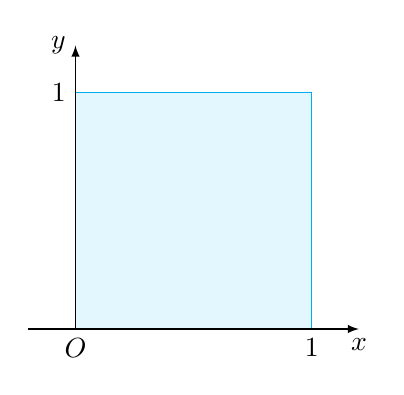
\begin{tikzpicture}[scale = 3]
            %画填充色快
            \filldraw[LightBlue] (0, 0) -- (0, 1) -- (1, 1) -- (1, 0) -- cycle;
            \draw[cyan] (0, 1) -- (1, 1) -- (1, 0);
            %标注坐标轴
            \draw[-latex] (-0.2, 0) -- (1.2, 0) node[below] {$x$};
            \draw[-latex] (0, 0) -- (0, 1.2) node[left] {$y$};
            \node[below] at (0,0) {$O$};
            %标注点
            \node[left] at (0, 1) {$1$};
            \node[below] at (1, 0)  {$1$};
        \end{tikzpicture}
    \end{center}
    得到
    $$
        \int_{0}^{1}\int_{0}^{1} kx^2y \,\mathrm{d}x\mathrm{d}y
        = \int_{0}^{1} kx^2 \mathrm{d}x \int_{0}^{1} y \,\mathrm{d}y
        = \int_{0}^{1} kx^2 \left(\left.\frac{y^2}{2}\right|_{0}^{1}\right) \mathrm{d}x
        = \left.\frac{k}{6}x^3\right|_{0}^{1}
        = 1,
    $$
    解得
    $$
        k=6.
    $$
    (2) 根据边缘概率密度的定义
    $$
        f_X(x) = \int_{-\infty}^{+\infty} f(x,y) \,\mathrm{d}y
        = \begin{dcases}
            \int_{0}^{1} 6x^2y \,\mathrm{d}y, & 0 \leqslant x \leqslant 1, \\
            0,                                & \text{其他}.
        \end{dcases}
        = \begin{cases}
            3x^2, & 0 \leqslant x \leqslant 1, \\
            0,    & \text{其他}.
        \end{cases}
    $$
    $$
        f_Y(y) = \int_{-\infty}^{+\infty} f(x,y) \,\mathrm{d}y
        = \begin{dcases}
            \int_{0}^{1} 6x^2y \,\mathrm{d}x, & 0 \leqslant y \leqslant 1, \\
            0,                                & \text{其他}.
        \end{dcases}
        = \begin{cases}
            2y, & 0 \leqslant y \leqslant 1, \\
            0,  & \text{其他}.
        \end{cases}
    $$
    (3) 新的积分区域如图所示
    \begin{center}
        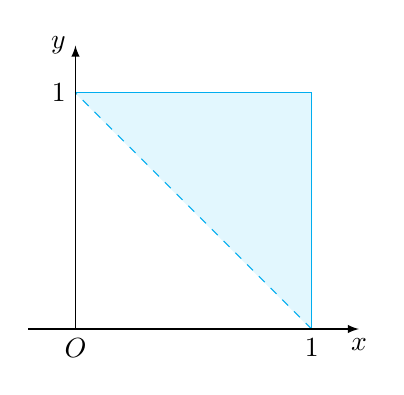
\begin{tikzpicture}[scale = 3]
            %画填充色快
            \filldraw[LightBlue] (0, 1) -- (1, 1) -- (1, 0) -- cycle;
            \draw[cyan, dashed] (1, 0) -- (0, 1);
            \draw[cyan] (0, 1) -- (1, 1) -- (1, 0);
            %标注坐标轴
            \draw[-latex] (-0.2, 0) -- (1.2, 0) node[below] {$x$};
            \draw[-latex] (0, 0) -- (0, 1.2) node[left] {$y$};
            \node[below] at (0,0) {$O$};
            %标注点
            \node[left] at (0, 1) {$1$};
            \node[below] at (1, 0)  {$1$};
        \end{tikzpicture}
    \end{center}
    根据概率密度的性质,得到
    $$
        P\{X+Y>1\}
        = \int_{0}^{1}\mathrm{d}x \int_{1-x}^1 6x^2y \,\mathrm{d}y
        = \int_{0}^{1} 3x^2\left[1-(1-x)^2\right] \,\mathrm{d}x
        = \frac{9}{10}.
    $$
\end{solution}
\end{document}